% Copyright 2013 Thomas Koenig, Alexander Michel, Michael Baumgart
%
% This file is part of NumericPlots.
%
% NumericPlots is free software: you can redistribute it and/or modify
% it under the terms of the GNU General Public License as published by
% the Free Software Foundation, either version 3 of the License, or
% any later version.
%
% NumericPlots is distributed in the hope that it will be useful,
% but WITHOUT ANY WARRANTY; without even the implied warranty of
% MERCHANTABILITY or FITNESS FOR A PARTICULAR PURPOSE.  See the
% GNU General Public License for more details.
%
% You should have received a copy of the GNU General Public License
% along with NumericPlots.  If not, see <http://www.gnu.org/licenses/>.


\documentclass[parskip]{scrartcl}

\usepackage[ansinew]{inputenc}
\usepackage[T1]{fontenc}
\usepackage{lmodern}

\usepackage{amsmath}
\usepackage{siunitx}
% \usepackage{floatbarrier}
% \usepackage{showexpl}
\usepackage{etex} % use e-TeX�s extended register set

% options for package:
% BW: black and white
% AxisStyle=<style>: set standard axis style ([Boxed], Frame, FrameI, None)
\usepackage[
	%BW,
  	xAxisStyle=Lower,
 	yAxisStyle=Left,
 	]{NumericPlots}
 
\usepackage[
	ps2pdf,							%% similar to dvips but redefines some macros for use with ps2pdf
	final,
	bookmarks=true,				%% if true, generate PDF bookmarks (requires two passes of pdflatex)
	bookmarksopen=false,			%% if true, show all PDF bookmarks expanded
	bookmarksnumbered=true,		%% if true, add the section numbers to the bookmarks
% 		linkbordercolor=acin_red,
% 		urlbordercolor=acin_red,
% 		citebordercolor=acin_red,
% 		filebordercolor=acin_red,
	pdfpagemode=UseOutlines, %% None, UseOutlines (=show bookmarks), UseThumbs (show thumbnails), FullScreen
%	breaklinks,
	pdfauthor = {Thomas Koenig Alexander Michel Michael Baumgart},
	pdftitle = {NumericPlots - plot numeric data with latex},
	pdfsubject = {},
	plainpages=false,
	hyperindex=true,
]{hyperref}

\usepackage{graphicx}

\definecolor{NumericPlotsCommands}{RGB}{0, 102, 153}
\usepackage{listings}
\lstset{language=[latex]tex,tabsize=2,basicstyle=\small\ttfamily,%
	numbers=none, numberstyle=\tiny,%
	breaklines=true, breakatwhitespace=false,%
	emptylines=*1,%
	columns=flexible,%
	keywordstyle=\color{black},commentstyle=\color{gray},%
	keywordstyle={[2]\color{NumericPlotsCommands}},%
	morekeywords={[2]setxAxis, setyAxis, NumericDataPlot, plotxAxis, plotyAxis,%
	NDPput,putExpX,putExpY,%
	putN,putNE,putE,putSE,putS,putSW,putW,putNW,%
	PutTickLabelYaxis,PutTickLabelXaxis,%
	NDPhline, NDPvline, NDPline, NDPhbox, NDPvbox, NDPbox,%
	LegendDefinition, LegLine,%
	StdLabelOption,StdTickLabelOption,%
	multilistplot, testframe}%
	}
 	
\title{NumericPlots - plot numeric data with latex}
\author{Thomas K\"{o}nig, Alexander Michel, Michael Baumgart}
\date{\today}

% \includeonly{TestPlots}
% \includeonly{TechnicalDetails}

% input DefineData here, as the examples from DefineData are used throughout the
% document (includeonly still works).
\def\IdentI{
	1.0 1.0e2
	1.1 11e1
	1.2 1.25e2
	1.3 110
	1.4 100
	1.5 90
	1.6 80
	}
\def\IdentII{
	1.0 125
	1.05 100
	1.1 75
	1.15 85
	1.2 90
	1.3 115
	1.4 130
	1.5 125
	1.6 120
	}
\def\LogData{
	6 6
	10 10
	20 20
	30 30
	40 40
	50 50
	60 60
	70 70
	80 80
	90 90
	100 100
	200 200
	300 300
	400 400
	500 500
	600 600
	700 700
	800 800
	900 900
	1000 1000
	1100 1100
	1200 1200
	1300 1300
	1400 1400
	1500 1500
}
% data written by export2latex
% date: 10-Mar-2010

\def\DataA{
2 58.828
3 56.353
4 58.817
5 55.814
6 56.713
7 52.671
8 56.493
9 48.933
10 52.068
11 45.674
12 48.869
13 48.317
14 49.677
15 62.636
16 51.374
17 48.876
}

\def\DataB{
2 62.894
3 59.824
4 59.908
5 56.158
6 54.775
7 50.489
8 50.897
9 44.732
10 44.923
11 39.731
12 39.663
13 37.731
14 36.13
15 38.342
16 30.646
17 28.224
}
\def\DataC{
    2.0000   52.5244
    3.0000   52.9925
    4.0000   52.7279
    5.0000   51.7954
    6.0000   50.4234
    7.0000   48.9477
    8.0000   47.7296
    9.0000   47.0674
   10.0000   47.1232
   11.0000   47.8834
   12.0000   49.1618
   13.0000   50.6454
   14.0000   51.9710
   15.0000   52.8140
   16.0000   52.9681
   17.0000   52.3955
}

\def\DataD{
2.0000   48.9294
    3.0000   47.7015
    4.0000   46.1762
    5.0000   44.5214
    6.0000   42.9193
    7.0000   41.5462
    8.0000   40.5534
    9.0000   40.0500
   10.0000   40.0916
   11.0000   40.6736
   12.0000   41.7318
   13.0000   43.1498
   14.0000   44.7715
   15.0000   46.4183
   16.0000   47.9090
   17.0000   49.0795
}

\def\DataE{
   2.0000   55.0918
    3.0000   57.2074
    4.0000   58.8597
    5.0000   59.9770
    6.0000   60.5465
    7.0000   60.6154
    8.0000   60.2864
    9.0000   59.7056
   10.0000   59.0472
   11.0000   58.4936
   12.0000   58.2160
   13.0000   58.3549
   14.0000   59.0052
   15.0000   60.2054
   16.0000   61.9334
   17.0000   64.1090
}

\def\DataF{
2 20.828
3 20.353
4 26.817
5 20.828
6 20.353
7 26.817
8 22.828
9 23.353
10 24.817
11 20.828
12 28.353
13 26.817
14 22.828
15 27.353
16 26.817
17 24.9
}

\def\DataG{
    2.0000   34.2537
    3.0000   33.1056
    4.0000   32.5301
    5.0000   32.3504
    6.0000   32.4343
    7.0000   32.6791
    8.0000   33.0000
    9.0000   33.3209
   10.0000   33.5657
   11.0000   33.6496
   12.0000   33.4699
   13.0000   32.8944
   14.0000   31.7463
   15.0000   29.7847
   16.0000   26.6776
   17.0000   21.9643
}


\def\DataDBhex{
2 93
3 87.09
4 80.44
5 74.57
6 68.55
7 63.55
8 57.9
9 53.86
10 49.4
11 46.09
12 42.51
13 39.17
14 35.98
15 32.39
16 30.25
17 28.53
}

\def\DataREShexint{
2 88.312
3 82.771
4 76.83
5 71.332
6 65.886
7 61.094
8 56.068
9 52.002
10 48.015
11 44.735
12 41.543
13 38.397
14 35.457
15 32.409
16 29.98
17 28.332
}



\begin{document}

% redefining the StdLabelOption and StdTickLabelOption applies to all following
% plots.
% \renewcommand{\StdLabelOption}{\LARGE}
% \renewcommand{\StdTickLabelOption}{\LARGE}

\maketitle

Plotting numeric data is a task which often has to be done for scientific
papers. In \LaTeX, however, it is only possible to include graphics created with
an external program. The pstricks-packages provide many commands to
generate graphics in \LaTeX. To generate simple graphics from numeric data,
however, it is difficult to use. This package provides a simpler interface for
the pstricks-package to plot numeric data.

The authors may be reached at
\href{mailto:numericplots@tikey.de}{numericplots@tikey.de}.

\tableofcontents

\part{Introduction}

Plotting numeric data is a task which often has to be done for scientific
papers. In \LaTeX, however, it is only possible to include graphics created with
an external program. The pstricks-packages provide very many commands to
generate graphics in \LaTeX. To generate simple graphics from numeric data,
however, it is difficult to use. This package provides a simpler interface for
the pstricks-package to plot numeric data.

NumericPlots is free software: you can redistribute it and/or modify
it under the terms of the GNU General Public License as published by
the Free Software Foundation, either version 3 of the License, or
any later version.

NumericPlots is distributed in the hope that it will be useful,
but WITHOUT ANY WARRANTY; without even the implied warranty of
MERCHANTABILITY or FITNESS FOR A PARTICULAR PURPOSE.  See the
GNU General Public License for more details.

You should have received a copy of the GNU General Public License
along with NumericPlots.  If not, see http://www.gnu.org/licenses/.

Copyright 2013 Thomas K\"{o}nig, Alexander Michel, Michael Baumgart


% \part{Using the package} -> in BasicFunctionality

% Copyright 2010 Thomas Koenig, Alexander Michel
%
% This file is part of NumericPlots.
%
% NumericPlots is free software: you can redistribute it and/or modify
% it under the terms of the GNU General Public License as published by
% the Free Software Foundation, either version 3 of the License, or
% any later version.
%
% NumericPlots is distributed in the hope that it will be useful,
% but WITHOUT ANY WARRANTY; without even the implied warranty of
% MERCHANTABILITY or FITNESS FOR A PARTICULAR PURPOSE.  See the
% GNU General Public License for more details.
%
% You should have received a copy of the GNU General Public License
% along with NumericPlots.  If not, see <http://www.gnu.org/licenses/>.

\part{Using the package}

\section{Basic Functionality}

The package NumericPlots\\
\verb+\usepackage{NumericPlots}+
\\
is intended to be used to plot numeric data which
may, e.g., be exported from Matlab by export2latex.m. The data must be defined
in the form
\lstinputlisting[lastline=9]{examples/DefineData}
where the first column contains the x, the second column the y-data.

\emph{Please note that the package relies on the \texttt{listplot}-command from
pstricks!}

\subsection{plots}


The easiest plot may be done by

\begin{minipage}[T]{0.45\linewidth}
	\lstinputlisting{examples/basic_EasyPlot}
\end{minipage}
\hspace{0.05\linewidth}
\begin{minipage}[T]{0.45\linewidth}
	\begin{NumericDataPlot}{\textwidth}{6.5cm}
	\setxAxis{xMin=-1, xMax=2, Dx=0.5, xO=0}
	\setyAxis{yMin=-50, yMax=150, Dy=25, yO=0}
	
	\plotxAxis{x-axis label}
	\plotyAxis{y-axis label}
	
	\listplot[style=StdLineStyA]{\IdentI}
\end{NumericDataPlot}
\end{minipage}

if you want to add a legend, you simply call

\begin{minipage}[T]{0.45\linewidth}
	\lstinputlisting{examples/basic_Legend}
\end{minipage}
\hspace{0.05\linewidth}
\begin{minipage}[T]{0.45\linewidth}
	\LegendDefinition{
	\LegLine{style=StdLineStyA} & IdentI
}
\end{minipage}

To plot multiple data in one plot call

\begin{minipage}[T]{0.45\linewidth}
	\lstinputlisting{examples/basic_MultipleData}
\end{minipage}
\hspace{0.05\linewidth}
\begin{minipage}[T]{0.45\linewidth}
	\centering
	\begin{NumericDataPlot}
   {\textwidth}{6.5cm}
	\setxAxis
	   {xMin=1, xMax=2, Dx=0.2}
	\setyAxis
	   {yMin=50, yMax=150, Dy=25}
	
	\plotxAxis{x-axis label}
	\plotyAxis{y-axis label}
	
	\listplot[style=StdLineStyA]
	   {\IdentI}
	\listplot[style=StdLineStyB]
	   {\IdentII}
	
	\putSE{\LegendDefinition{
		\LegLine{style=StdLineStyA} & IdentI \\
		\LegLine{style=StdLineStyB} & IdentII
	}}
\end{NumericDataPlot}
\end{minipage}


\subsection{Label and TickLabels}

The commands \texttt{plotxAxis} and \texttt{plotyAxis} take the options
\texttt{NoLabel}, \texttt{NoTicks}, \texttt{NoTickLabel} as well as
\texttt{LabelOption} and \texttt{TickLabelOption} which may be used to eliminate
or change the look of the labels.

Standard values for \texttt{LabelOption} and \texttt{TickLabelOption} may be set\\
by \verb|\newcommand{\StdLabelOption}{\color{blue}|\\
and \verb|\newcommand{\StdTickLabelOption}{\small}|.

The option \texttt{LabelSep} may be used for \verb|\plotxAxis| and
\verb|\plotyAxis| to set the seperation between the axis and the label. Standard
value is \verb|\baselineskip+1ex| for the x-label and \verb|7ex| for the
y-label.

\begin{minipage}[T]{0.45\linewidth}
	\lstinputlisting{examples/basic_Labels}
\end{minipage}
\hspace{0.05\linewidth}
\begin{minipage}[T]{0.45\linewidth}
	\begin{NumericDataPlot}{\textwidth}{6.5cm}
	\setxAxis{xMin=1, xMax=1.6, Dx=0.1, DDx=0.2}
	\setyAxis{yMin=75, yMax=130, Dy=12.5}
	
	\plotxAxis
	[LabelOption=\LARGE,%
	TickLabelOption=\color{red},%
	LabelSep=40pt]
	{x-axis label}
	\plotyAxis
	[NoLabel, NoTicks, NoTickLabel]
	{y-axis label}
	
	\listplot[style=StdLineStyA]{\IdentI}
	\listplot[style=StdLineStyB]{\IdentII}
	
\end{NumericDataPlot}
\end{minipage}

It is furthermore possible to change the position and the rotation of the labels
and tick labels, see the example in section \ref{sec:Details:Labels}.

It is also possible to put single tick labels, see the example in section
\ref{sec:Details:Labels}.

\subsection{Place ``Objects'' in the plot.}\label{sec:PlaceObjects}

There are basically two different options to place objects in the plot. To
understand the difference one has to keep in mind that the axis have two
different coordinate systems. One is the system defined by xMin, xMax, yMin and
yMax (refered to as ``DataCoordinateSystem''), the other ist the system defined
by xCoordMin, xCoordMax, yCoordMin and yCoordMax (refered to as
``PictureCoordinateSystem''), see section \ref{sec:MultiplePlots}.

It is now possible to place stuff in the graph with the DataCoordinates with the
command NDPput, see the following example.

\begin{minipage}[T]{0.45\linewidth}
	\lstinputlisting{examples/basic_PlaceObjects}
\end{minipage}
\hspace{0.05\linewidth}
\begin{minipage}[T]{0.45\linewidth}
	\begin{NumericDataPlot}
   {\textwidth}{6.5cm}
	\setxAxis
	   {xMin=1, xMax=2, Dx=0.2}
	\setyAxis
	   {yMin=50, yMax=150, Dy=25}
	
	\plotxAxis[LabelPos=1, LabelRefPt=tr]%
		{x-axis label}
	\plotyAxis[NoLabel]{}
	
	\listplot[style=StdLineStyA]
	   {\IdentI}
	
	% put some stuff somewhere
	\NDPput[x=1.2, y=75, RefPoint=br]{text}
	\NDPput[x=1.2, y=100, Rot=45]{$a^2+b^2$}
	
	% or put nodes...
	\NDPput[x=1.6, y=100]{\pnode{A}}
	\NDPput[x=1.8, y=150]{\pnode{B}}
	% ...and draw a line between them
	\ncline{A}{B}
	% .. with text
	\naput{$e^2$}
	
	% or put the legend at a specific position
	\NDPput[x=1.8, y=75]{\LegendDefinition{
		\LegLine{style=StdLineStyA} & IdentI
	}}
\end{NumericDataPlot}
\end{minipage}


For convenience the commands \verb|\putXX{object}| where
$XX\in\left(N,S,E,W,NW,NE,SW,SE\right)$ are defined to place something in the
North, South,\ldots, SouthEast corner of the plot. Also, the command
\verb|\putExpY{xx}| and \verb|\putExpX{xx}| may be used to place exponents at
the axes.

\begin{minipage}[T]{0.45\linewidth}
	\lstinputlisting[firstline=14,lastline=24]{examples/basic_PlaceObjectsII}
\end{minipage}
\hspace{0.05\linewidth}
\begin{minipage}[T]{0.45\linewidth}
		\begin{NumericDataPlot}
	   {\textwidth}{6.5cm}
		\setxAxis
		   {xMin=1, xMax=1.6, Dx=0.2}
		\setyAxis
		   {yMin=50, yMax=150, Dy=25}
		
		\plotxAxis{x-axis label}
		\plotyAxis[NoLabel]{}
		
		\listplot[style=StdLineStyA]
		   {\IdentI}
		
		\putExpY{$\times 10^{-3}$}
		\putExpX{$\times 10^{-6}$}
		
		\putN{N}
		\putS{S}
		\putW{W}
		\putE{E}
		\putNW{NW}
		\putNE{NE}
		\putSW{SW}
		\putSE{SE}
	\end{NumericDataPlot}
\end{minipage}

Alternatively, stuff can be placed
within the plot with \verb|\rput|.


\begin{minipage}[T]{0.5\linewidth}
	\lstinputlisting[firstline=14,lastline=28]{examples/basic_UseRput}
\end{minipage}
\begin{minipage}[T]{0.5\linewidth}
	\begin{NumericDataPlot}
   {\textwidth}{6.5cm}
	\setxAxis
	   {xMin=1, xMax=1.6, Dx=0.2}
	\setyAxis
	   {yMin=50, yMax=150, Dy=25}
	
	\plotxAxis{x-axis label}
	\plotyAxis[NoLabel]{}
	
	\listplot[style=StdLineStyA]
	   {\IdentI}
	
	% put text in the middle of the plot
	\rput{45}(500,500){text}
	% put a formula in the lower left corner
	\rput[bl](0,0){$a^2+b^2=c^2$}
	
	% or put nodes...
	\NDPput[x=1.2, y=125]{\pnode{A}}
	\rput(750,900){\Rnode{B}{peak}}
	% ...and draw a line between them
	\ncline{<-}{A}{B}
	
	% or put the legend at a specific position
	\rput{-45}(750,250){\LegendDefinition{
		\LegLine{style=StdLineStyA} & IdentI
	}}
\end{NumericDataPlot}
\end{minipage}


% =================================
% |								  |
% |     Linestyles and colors     |
% |								  |
% =================================

\subsection{Linestyles and colors}

While using the package, there are predefined linestyles which may be used:

\begin{minipage}{0.55\linewidth}
	\centering
	\small
	
	\begin{NumericDataPlot}[lly=1cm,llx=1cm,urx=0.25cm,ury=0.25cm]{\linewidth}{0.85\linewidth}
		\setxAxis{xMin=2, xMax=17, xO=5, Dx=4}
		\setyAxis{yMin=20, yMax=70, yO=20, Dy=20}
			
        \plotxAxis[NoLabel, AxisStyle=Boxed]{}
        \plotyAxis[NoLabel, AxisStyle=Boxed]{}

		\listplot[style=StdLineStyA]{\DataA}
		\listplot[style=StdLineStyB]{\DataB}
		\listplot[style=StdLineStyC]{\DataC}
		\listplot[style=StdLineStyD]{\DataD}
		\listplot[style=StdLineStyE]{\DataE}
		\listplot[style=StdLineStyF]{\DataF}
		\listplot[style=StdLineStyG]{\DataG}
	\end{NumericDataPlot}
\end{minipage}
\begin{minipage}{0.4\linewidth}
	\centering
	\LegendDefinition{
		\LegLine{style=StdLineStyA} & StdLineStyA \\
		\LegLine{style=StdLineStyB} & StdLineStyB \\
		\LegLine{style=StdLineStyC} & StdLineStyC \\
		\LegLine{style=StdLineStyD} & StdLineStyD \\
		\LegLine{style=StdLineStyE} & StdLineStyE \\
		\LegLine{style=StdLineStyF} & StdLineStyF \\
		\LegLine{style=StdLineStyG} & StdLineStyG \\
	}
\end{minipage}

When using the package option \texttt{BW} the standard line styles will be
replaced by their black and white counterparts:

\begin{minipage}{0.6\linewidth}
	\centering
	\small
	
	\begin{NumericDataPlot}[lly=1cm,llx=1cm,urx=0.25cm,ury=0.25cm]{\linewidth}{0.85\linewidth}
		\setxAxis{xMin=2, xMax=17, xO=5, Dx=4}
		\setyAxis{yMin=20, yMax=70, yO=20, Dy=20}
			
        \plotxAxis[NoLabel, AxisStyle=Boxed]{}
        \plotyAxis[NoLabel, AxisStyle=Boxed]{}

		\listplot[style=BWStdLineStyA]{\DataA}
		\listplot[style=BWStdLineStyB]{\DataB}
		\listplot[style=BWStdLineStyC]{\DataC}
		\listplot[style=BWStdLineStyD]{\DataD}
		\listplot[style=BWStdLineStyE]{\DataE}
		\listplot[style=BWStdLineStyF]{\DataF}
		\listplot[style=BWStdLineStyG]{\DataG}
	\end{NumericDataPlot}
\end{minipage}
\begin{minipage}{0.4\linewidth}
	\centering
	\LegendDefinition{
		\LegLine{style=BWStdLineStyA} & BWStdLineStyA \\
		\LegLine{style=BWStdLineStyB} & BWStdLineStyB \\
		\LegLine{style=BWStdLineStyC} & BWStdLineStyC \\
		\LegLine{style=BWStdLineStyD} & BWStdLineStyD \\
		\LegLine{style=BWStdLineStyE} & BWStdLineStyE \\
		\LegLine{style=BWStdLineStyF} & BWStdLineStyF \\
		\LegLine{style=BWStdLineStyG} & BWStdLineStyG \\
	}
\end{minipage}

For values which are nearly the same (reference and measurement, e.g.) the
following line styles may be used:

\begin{minipage}{0.58\linewidth}
	\centering
	\small
	
	\begin{NumericDataPlot}[lly=1cm,llx=1cm,urx=0.25cm,ury=0.25cm]{\linewidth}{0.85\linewidth}
		\setxAxis{xMin=2, xMax=17, xO=5, Dx=4}
		\setyAxis{yMin=20, yMax=70, yO=20, Dy=20}
			
        \plotxAxis[NoLabel, AxisStyle=Boxed]{}
        \plotyAxis[NoLabel, AxisStyle=Boxed]{}

		\listplot[style=StdLineStyX]{\DataC}
		\listplot[style=StdLineStyY]{\DataC}
		
		\listplot[style=BWStdLineStyX]{\DataD}
		\listplot[style=BWStdLineStyY]{\DataD}
	\end{NumericDataPlot}
\end{minipage}
\begin{minipage}{0.38\linewidth}
	\centering
	\LegendDefinition{
		\LegLine{style=StdLineStyX} & StdLineStyX \\
		\LegLine{style=StdLineStyY} & StdLineStyY \\
		\LegLine{style=BWStdLineStyX} & BWStdLineStyX \\
		\LegLine{style=BWStdLineStyY} & BWStdLineStyY \\
	}
\end{minipage}

It is, of course, possible to redefine the available linestyles or to define new
linestyles.

\begin{minipage}[T]{0.48\linewidth}
	\lstinputlisting[firstline=4,lastline=26]{examples/basic_UserLinestyles}
\end{minipage}
\begin{minipage}[T]{0.48\linewidth}
	\begin{NumericDataPlot}
   {\textwidth}{6.5cm}

   \definecolor{MyColor}{cmyk}{0.6 0.21 1.0 0.2}
   \newpsstyle{MyLine}{linecolor=MyColor, linewidth=2pt, linestyle=dashed,
   dash=1pt 1pt 4pt 1pt 1pt 3pt, dotstyle=*, showpoints=true, dotsize=5pt}
   \newpsstyle{MyLineA}{linecolor=blue, linestyle=dotted, dotstyle=asterisk,
   showpoints=true}

	\setxAxis
	   {xMin=1, xMax=1.6, Dx=0.2}
	\setyAxis
	   {yMin=50, yMax=150, Dy=25}
	
	\plotxAxis[NoLabel]{}
	\plotyAxis[NoLabel]{}
	
	\listplot[style=MyLine]
	   {\IdentI}
	\listplot[style=MyLineA]
	   {\IdentII}
	
	\putSE{\LegendDefinition{
		\LegLine{style=MyLine} & IdentI\\
		\LegLine{style=MyLineA} & IdentII
	}}
\end{NumericDataPlot}
\end{minipage}



% =================================
% |								  |
% |            Legend             |
% |								  |
% =================================

\subsection{Legend}

The legend may be created with \verb|\LegendDefinition|. The command takes the
two optional arguments \texttt{nrCols} and \texttt{LabelOrientation=[l|c|r]}.
The mandatory argument is the definition of a table as demonstrated in the
follwing examples.

\begin{minipage}[T]{0.5\linewidth}
	\lstinputlisting{examples/basic_LegendI}
\end{minipage}
\hspace{1ex}
\begin{minipage}[T]{0.4\linewidth}
	\LegendDefinition{
	\LegLine{style=StdLineStyA} & IdentI\\
	\LegLine{style=StdLineStyB, linewidth=3pt} & second legend
}
\end{minipage}

\begin{minipage}[T]{0.5\linewidth}
	\lstinputlisting{examples/basic_LegendII}
\end{minipage}
\hspace{1ex}
\begin{minipage}[T]{0.4\linewidth}
		\newpsstyle{LegendBoxStyle}%
		{framearc=0.2, fillstyle=solid, fillcolor=yellow, opacity=0.2}
	\LegendDefinition[nrCols=2]{
		\LegLine{style=StdLineStyA} & IdentI &
		\LegLine{style=StdLineStyB, linewidth=3pt} & legend 2
	}
	\newpsstyle{LegendBoxStyle}%
		{fillstyle=solid, fillcolor=white}
\end{minipage}

\begin{minipage}[T]{0.5\linewidth}
	\lstinputlisting{examples/basic_LegendIII}
\end{minipage}
\hspace{1ex}
\begin{minipage}[T]{0.4\linewidth}
	\LegendDefinition[LabelOrientation=c]{
	\LegLine{style=StdLineStyA} & IdentI\\
	\LegLine{style=StdLineStyB, linewidth=3pt} & second legend\\
	\LegLine{style=StdLineStyC} & whatever this data is\ldots\\
	\LegLine{style=StdLineStyD} & and more data\\
	\LegDot{style=StdLineStyC, plotstyle=dots} & plotstyle=dots
}
\end{minipage}


\subsection{Add Lines to the Plot}

Horizontal and vertical lines may be added to the plot with the commands
\verb|\NDPhline{coord}|, \verb|\NDPvline{coord}| and \verb|\NDPline{coord}|. It is also possible to put
nodes and draw lines between them, see section \ref{sec:PlaceObjects}.

\begin{minipage}[T]{0.5\linewidth}
	\lstinputlisting[firstline=14,lastline=17]{examples/basic_Lines}
\end{minipage}
\hspace{1ex}
\begin{minipage}[T]{0.4\linewidth}
	\begin{NumericDataPlot}
   {\textwidth}{6cm}
	\setxAxis
	   {xMin=1, xMax=1.6, Dx=0.2}
	\setyAxis
	   {yMin=50, yMax=150, Dy=25}
	
	\plotxAxis[NoLabel]{}
	\plotyAxis[NoLabel]{}
	
	\listplot[style=StdLineStyA]
	   {\IdentI}
	
	\NDPhline[linecolor=LineColorD]{73}
	\NDPvline[linecolor=LineColorE, %
		linestyle=dashed]{1.5}
	\NDPline[linecolor=red]{1.1}{75}{1.3}{125}
\end{NumericDataPlot}
\end{minipage}


\subsection{Add Boxes to the Plot}

Horizontal and vertical boxes may be added to the plot with the commands
\verb|\NDPhbox{coord}|, \verb|\NDPvbox{coord}| and \verb|\NDPbox{coord}|. It is also possible to put
nodes and draw lines between them, see section \ref{sec:PlaceObjects}.

\begin{minipage}[T]{0.5\linewidth}
	\lstinputlisting[firstline=11,lastline=21]{examples/basic_Boxes}
\end{minipage}
\hspace{1ex}
\begin{minipage}[T]{0.4\linewidth}
	\begin{NumericDataPlot}
   {\textwidth}{6cm}
	\setxAxis
	   {xMin=1, xMax=1.6, Dx=0.2}
	\setyAxis
	   {yMin=50, yMax=150, Dy=25}
	
	\plotxAxis[NoLabel]{}
	\plotyAxis[NoLabel]{}
			
	\NDPhbox[fillstyle=solid,fillcolor = green]%
            {75.0}{100.0}%

	\listplot[style=StdLineStyA] {\IdentI}

	\NDPvbox[fillstyle=solid,fillcolor=red]
            {1.4}{1.5}

    \NDPbox[fillstyle=solid,%
        fillcolor=orange, opacity=0.2, linestyle=none]%
		{1.1}{60}{1.15}{130}
\end{NumericDataPlot}
\end{minipage}


\subsection{Grid}

As shwon in the example below, it is possible to plot a fine grid but not have a
tick label at each of the grid lines. While the options \texttt{Dx} and
\texttt{Dy} define the distance between the grid lines, the options \texttt{DDx}
and \texttt{DDy} define the distance between the tick labels. If \texttt{DDx} or
\texttt{DDy} are not set, they take the values of \texttt{Dx} and \texttt{Dy}. 

One may choose not to plot the grid with
the option \texttt{NoGrid} for the commands \verb|\plotxAxis| and \verb|\plotyAxis|.

If the grid is plottet with the axis it may happen that the grid is plottet over
the axis. To avoid this, plot the grid first and then plot the axis as shown.

\begin{minipage}[T]{0.5\linewidth}
	\lstinputlisting{examples/basic_Grid}
\end{minipage}
\hspace{1ex}
\begin{minipage}[T]{0.4\linewidth}
	\begin{NumericDataPlot}
   {\textwidth}{6.5cm}
	\setxAxis{xMin=1, xMax=1.6, Dx=0.1, DDx=0.2}
	\setyAxis{yMin=50, yMax=150, Dy=12.5, DDy=25}
	
	\plotxGrid
	\plotyGrid
	\plotxAxis[NoLabel, NoGrid, AxisStyle=Boxed]{}
	\plotyAxis[NoLabel, NoGrid, AxisStyle=Boxed]{}
	
	\listplot[style=StdLineStyA]{\IdentI}
	
\end{NumericDataPlot}
\end{minipage}



\subsection{Logarithmic axes}


\begin{minipage}[T]{0.5\linewidth}
	\lstinputlisting{examples/basic_LogarithmicI}
\end{minipage}
\hspace{1ex}
\begin{minipage}[T]{0.4\linewidth}
	\begin{NumericDataPlot}{\textwidth}{6.5cm}
	\setxAxis{xMin=6, xMax=2500, xLog}
	\setyAxis{yMin=0, yMax=2500, Dy=500}
	\plotxAxis{}
	\plotyAxis{}
	
	\listplot{\LogData}
\end{NumericDataPlot}
\end{minipage}


\begin{minipage}[T]{0.5\linewidth}
	\lstinputlisting{examples/basic_LogarithmicII}
\end{minipage}
\hspace{1ex}
\begin{minipage}[T]{0.4\linewidth}
	\begin{NumericDataPlot}{\textwidth}{6.5cm}
	\setxAxis{xMin=1, xMax=1500, xLog}
	\setyAxis{yMin=1, yMax=1500, yLog}
	\plotxAxis{}
	\plotyAxis{}
	
	\listplot{\LogData}
\end{NumericDataPlot}
\end{minipage}


\begin{minipage}[T]{0.5\linewidth}
	\lstinputlisting{examples/basic_LogarithmicIII}
\end{minipage}
\hspace{1ex}
\begin{minipage}[T]{0.4\linewidth}
	\begin{NumericDataPlot}{\textwidth}{6.5cm}
	\setxAxis{xMin=1, xMax=1500, xLog, xLogNoSubGrid}
	\setyAxis{yMin=1, yMax=1500, yLog, yLogNoSubGrid}
	\plotxAxis{}
	\plotyAxis{}
	
	\listplot{\LogData}
\end{NumericDataPlot}
\end{minipage}


\subsection{plots with holes}

If plotting data, one might not want to plot some part of this data, e.g. if
only the data in a certain y-range is interesting. If one chooses to eliminate the
invalid data either by using \verb+yStart+ or \verb+yEnd+ or by eliminating the
data before the export, pstricks will always connect the last valid point of an
interval with the first valid point of the next interval. In Matlab e.g.,
invalid data (NaN) is just ignored. This behavior is also possible with NumericPlots and
export2latex. If export2latex is called with data which contains NaN and with
the option.NaNsplit=true, it will split the data in several intervals and append
a consecutive number to the identifier for each interval. The exported yMax,
yMin values etc. will still be valid for the whole data-vector. The exported
data might look like:

\begin{verbatim}
\expandafter\def\csname DataIdentNrRanges\endcsname{3}
\expandafter\def\csname DataIdent1\endcsname{
560.00 5.40
...
574.72 6.25
}

\expandafter\def\csname DataIdent2\endcsname{
588.73 4.78
...
609.53 12.09
}


\expandafter\def\csname DataIdent3\endcsname{
620.56 27.81
...
649.56 27.32
}
\end{verbatim}


\expandafter\def\csname DataIdentNrRanges\endcsname{3}
\expandafter\def\csname DataIdent1\endcsname{
560.00 5.40
560.30 6.25
560.59 4.74
560.90 6.25
561.60 5.18
561.65 6.25
561.70 4.73
562.60 4.75
562.63 6.06
563.75 6.12
563.75 5.00
564.50 6.25
564.76 4.71
564.90 4.88
565.51 6.25
565.63 5.00
566.13 5.69
566.61 6.78
567.10 4.88
567.60 4.89
567.66 6.25
568.30 4.88
568.31 6.25
569.10 4.77
569.51 6.25
569.60 6.13
570.35 4.85
570.63 6.25
570.71 5.00
571.30 4.64
571.31 6.25
572.30 4.66
572.62 6.06
572.90 5.00
572.93 5.61
573.68 5.00
574.11 6.25
574.66 4.76
574.72 6.25
}

\expandafter\def\csname DataIdent2\endcsname{
588.73 4.78
588.90 6.15
589.50 4.76
589.67 4.90
589.74 6.25
590.66 5.96
590.73 4.55
591.25 6.25
591.69 4.68
592.10 4.91
592.31 6.25
593.20 6.25
593.55 5.36
593.64 4.79
593.74 6.25
594.64 4.74
594.75 6.11
595.25 4.67
595.31 6.12
596.00 5.84
596.30 11.90
597.10 10.69
597.20 12.00
597.69 12.00
598.15 10.00
598.50 11.97
598.67 10.00
599.31 10.00
599.69 11.91
600.13 12.22
600.79 10.79
600.83 10.31
600.86 11.72
601.74 10.56
601.80 11.25
602.78 11.98
602.94 10.00
603.72 12.08
603.94 10.00
604.54 10.00
604.70 11.96
605.14 11.25
605.24 10.83
605.69 11.92
605.80 10.00
606.70 11.72
607.03 10.00
607.49 11.15
607.54 10.00
608.23 12.15
608.72 10.00
609.30 10.87
609.53 12.09
}

\expandafter\def\csname DataIdent3\endcsname{
620.56 27.81
620.78 26.25
620.85 27.80
621.56 27.32
621.74 27.78
622.00 27.32
622.74 26.36
623.08 28.75
623.31 27.79
623.71 26.31
624.05 27.32
624.65 27.79
625.18 27.83
625.45 27.35
625.95 27.74
626.28 27.30
626.75 26.34
626.88 27.81
627.54 28.75
627.72 26.38
628.23 27.29
628.36 27.74
628.88 26.25
629.28 27.82
629.78 28.84
629.93 27.32
631.13 26.27
631.22 27.76
631.94 28.75
631.98 27.33
632.54 26.25
632.66 27.78
632.89 27.29
633.33 28.88
633.76 26.45
633.94 27.85
634.76 26.33
635.14 27.74
635.68 27.82
635.84 26.35
636.08 27.84
636.46 27.34
637.04 27.74
637.19 27.32
637.70 27.34
638.31 27.84
638.50 27.78
638.65 27.33
639.45 27.79
639.83 26.34
640.03 27.38
640.68 27.83
641.45 27.31
641.50 27.77
642.08 27.80
642.18 27.32
642.76 27.93
642.86 26.25
643.75 27.32
643.91 27.76
644.38 27.30
644.74 27.83
645.06 27.37
645.08 27.80
645.80 28.80
646.13 26.47
646.76 26.57
647.09 27.81
647.26 27.83
647.98 26.25
648.20 27.33
648.34 28.75
648.93 28.91
649.56 27.32
}

This data can then easily be plotted using the command\\
\verb+\multilistplot{<options>}{<Identifier>}+\footnote{Please notice, that the
first argument of multilistplot is a mandatory argument. Also notice, that the
second argument ist only the name of the data including ``Data'' but not the
command as it would be for the listplot command}.
The command will call\\
\verb+\listplot[<options>]{\<Identifier>}+ for each of
the intervals. The first argument is directly passed to the listplot command which is part of the
pstricks package. The second argument is the identifier of the data that should
be plotted.

\begin{minipage}[T]{0.5\linewidth}
	\lstinputlisting{examples/basic_PlotWHoles}
\end{minipage}
\hspace{1ex}
\begin{minipage}[T]{0.4\linewidth}
	\begin{NumericDataPlot}{\textwidth}{6.5cm}
	\setxAxis{xMin=560, xMax=650, Dx=20}
	\setyAxis{yMin=4, yMax=30, Dy=5, yO=5}
	\plotxAxis{}
	\plotyAxis{}
	
	\multilistplot{style=StdLineStyA}{DataIdent}
\end{NumericDataPlot}
\end{minipage}



% Copyright 2010 Thomas Koenig, Alexander Michel
%
% This file is part of NumericPlots.
%
% NumericPlots is free software: you can redistribute it and/or modify
% it under the terms of the GNU General Public License as published by
% the Free Software Foundation, either version 3 of the License, or
% any later version.
%
% NumericPlots is distributed in the hope that it will be useful,
% but WITHOUT ANY WARRANTY; without even the implied warranty of
% MERCHANTABILITY or FITNESS FOR A PARTICULAR PURPOSE.  See the
% GNU General Public License for more details.
%
% You should have received a copy of the GNU General Public License
% along with NumericPlots.  If not, see <http://www.gnu.org/licenses/>.


\section{Multiple plots in one picture}\label{sec:MultiplePlots}

xPicMin, xPicMax, yPicMin and yPicMax are the inner coordinates of one picture.
The position of the axes are defined in this coordinate system via xCoordMin,
xCoordMax, yCoordMin and yCoordMax.

Example:


\lstinputlisting[firstline=8]{examples/multiplots_exampleI}

% define linestyles
\newpsstyle{Database}{linecolor=LineColorA, linestyle=none, dotstyle=*,
showpoints=true, dotsize=5pt}
\newpsstyle{Result}{linecolor=LineColorB, linestyle=none, dotstyle=+,
showpoints=true, dotsize=10pt}

\begin{center}
	\begin{NumericDataPlot}[xPicMin=0, xPicMax=1050,
	yPicMin=0, yPicMax=1450]{\textwidth}{0.85\textheight}
		
		% --- definition of the axis and the grid ---
		% set the axis of the lower left corner
		\setxAxis{xMin=2, xMax=17, Dx=4, xCoordMin=0, xCoordMax=500}
		\setyAxis{yMin=20, yMax=70, Dy=20, yCoordMin=0, yCoordMax=500}
		
		% plot the axis of the lower left corner
		\plotxAxis{Stichnummer}
		\plotyAxis{$F_{roll}$ in $\si{\mega\newton}$}





		\listplot[style=Database]{\DataA}
		\listplot[style=Result]{\DataB}
		\listplot[style=StdLineStyC]{\DataC}
		\listplot[style=StdLineStyD]{\DataD}
		\listplot[style=StdLineStyE]{\DataE}
		\listplot[style=StdLineStyF]{\DataF}
		\listplot[style=StdLineStyG]{\DataG}
		
		% set the y-axis for the plot in the middle of the left side
		% x-axis remains the same
		\setyAxis{yMin=20, yMax=70, Dy=20, yCoordMin=550, yCoordMax=1050}
		% plot the axis (x-axis without ticklabels)
		\plotxAxis[NoTickLabel,LabelSep=1ex]{a) Ein plot}
		\plotyAxis{$F_{roll}$ in $\si{\mega\newton}$}

		\listplot[style=Database]{\DataA}
		\listplot[style=Result]{\DataB}
		
		% set axis for the plot at the right side
		\setxAxis{xMin=2, xMax=17, Dx=4, xCoordMin=600, xCoordMax=1050}
		\setyAxis{yMin=20, yMax=70, Dy=10, yCoordMin=0, yCoordMax=1050}
		
		% plot the axis at the right side (y-axis without label)
		\plotxAxis{Stichnummer}
		\plotyAxis[NoLabel]{$F_{roll}$ in $\mega\newton$}

		\listplot[style=Database]{\DataA}
		\listplot[style=Result]{\DataB}
		\listplot[style=StdLineStyC]{\DataC}
		\listplot[style=StdLineStyD]{\DataD}
		\listplot[style=StdLineStyE]{\DataE}
		\listplot[style=StdLineStyF]{\DataF}
		\listplot[style=StdLineStyG]{\DataG}
		
		% set the axis for the plot at the top
		\setxAxis{xMin=8, xMax=17, Dx=1, xCoordMin=0, xCoordMax=1050}
		\setyAxis{yMin=35, yMax=65, Dy=10, yO=40, yCoordMin=1150, yCoordMax=1450}
		
		% plot the axis for the plot at the top
		\plotxAxis[NoLabel]{Stichnummer}
		\plotyAxis[NoLabel]{$F_{roll}$ in $\mega\newton$}

		% plot only part of the data
		\listplot[style=Database, xStart=11, xEnd=17]{\DataA}
		\listplot[style=Result, xStart=8, xEnd=13]{\DataB}
		
	\end{NumericDataPlot}
	
	% put legend outside of the plot
	\LegendDefinition[nrCols=1, LabelOrientation=r]{
		\LegLine{style=Database} & Werte aus der Datenbank \\
		\LegLine{style=Result} & Modell}
\end{center} 


An example with different y-axes on the left and on the right side:

\lstinputlisting{examples/multiplots_exampleII}

\newpsstyle{Database}{linecolor=LineColorA, linestyle=none, dotstyle=*,
showpoints=true, dotsize=5pt}
\newpsstyle{Result}{linecolor=LineColorB, linestyle=none, dotstyle=+,
showpoints=true, dotsize=10pt}

\begin{NumericDataPlot}{\textwidth}{0.25\textheight}
		
	% --- definition of the axis and the grid ---
	\setxAxis{xMin=2, xMax=17, Dx=4}
	\setyAxis{yMin=20, yMax=70, Dy=20}
	
	% plot the axis of the lower left corner
	\plotxAxis{Stichnummer}
	\plotyAxis{$F_{roll}$ in $\si{\mega\newton}$}

	\listplot[style=Database]{\DataA}
	
	% define a second y-axis 
	\setyAxis{yMin=40, yMax=90, Dy=20}
	\plotyAxis[AxisStyle=Right, NoGrid]{$F_{roll}$}
	
	\listplot[style=Result]{\DataA}
	
\end{NumericDataPlot}


It is also possible to rotate the labels of the axes (LabelRot and LabelRefPt
have to be set after AxisStyle!):

\lstinputlisting[firstline=12, lastline=20]{examples/multiplots_exampleIII}

\newpsstyle{Database}{linecolor=LineColorA, linestyle=none, dotstyle=*,
showpoints=true, dotsize=5pt}
\newpsstyle{Result}{linecolor=LineColorB, linestyle=none, dotstyle=+,
showpoints=true, dotsize=10pt}

\begin{NumericDataPlot}{\textwidth}{0.25\textheight}
		
	% --- definition of the axis and the grid ---
	\setxAxis{xMin=2, xMax=17, Dx=4}
	\setyAxis{yMin=20, yMax=70, Dy=20}
	
	% plot the axis of the lower left corner
	\plotxAxis[LabelRot=15]{Stichnummer}
	\plotyAxis[LabelRot=30, LabelRefPt=tr]{$F_{roll}$ in $\si{\mega\newton}$}

	\listplot[style=Database]{\DataA}
	
	% define a second y-axis 
	\setyAxis{yMin=40, yMax=90, Dy=20}
	\plotyAxis[AxisStyle=Right, NoGrid, LabelRot=90]{$F_{roll}$}
	
	\listplot[style=Result]{\DataA}
	
\end{NumericDataPlot}



\section{Matlab Support}


\subsection{export2latex.m}
The function \texttt{export2latex(data, filename, [options])} may be used to
export data from Matlab to be used with NumericPlots.sty. The function takes the
two parameters data and filename, where filename is the name of the file where
the data should be stored with full path but without extension. Data is a
structure with the three entries x, y, and ident, where x are the x-data, y the
y-data and ident is an identifier to have access to the data in Latex. To access
the data in Latex the command \verb+\Data<ident>+ is used.

The parameter data may be provided as an 1xK array if each entry of the array is
a structure with the entries x, y and ident. There may be an additional entry
descr.
\begin{itemize}
  \item data(1,i).x = $X_i$
  \item data(1,i).y = $Y_i$
  \item data(1,i).ident = Identifier
  \item (data(1,i).descr = Description)
  \item (data(1,i).group = GroupNr)
\end{itemize}
Identifier must be a valid Latex command name, which basically means it must be
a string without numbers.

For every entry of data, $X$ and $Y$ must be arrays of the same size
$M\text{x}N$. If $M>1$, each column of the array is exported to the file and the
identifier is expanded by the roman representation of the column number.

It might be useful to do a \texttt{interp1} before exporting the data to get
smaller files and to use less of \TeX's memory. ($\rightarrow$ script
Patrick?!?)

The optional parameter \texttt{options} might be used to control which
additional information is provided in the output file.
\begin{itemize}
	\item \texttt{options.DataBoundaries} [true] If set to true, the output file
	contains the commands \verb+\DataXmin+, \verb+\DataXmax+, \verb+\DataYmin+ and
	\verb+\DataYmax+ which may be used to define the axis.
	\item \texttt{options.AxisBoundaries} [false] If set to true, the output file
	contains the commands \verb+\DataXminAxis+, \verb+\DataXmaxAxis+,
	\verb+\DataYminAxis+ and \verb+\DataYmaxAxis+ which may be used to define the
	axis. In contrary to the DataBoundaries the AxisBoundaries add an additional
	gap of \texttt{options.AxisBoundariesGap} [10] percent of the full scale to
	the data boundaries such that the plot doesn't touch the axis.
	\item \texttt{options.SuppressWarning} [false] suppresses the warning about
	max/min values being to close together
	\item \texttt{options.precision} [empty] how many decimal places should be
	printed for x and y values. Will be calculated automatically if left empty.
	\item \texttt{options.NaNsplit [false]} if true, the data will be split at NaN
	values. See \verb+\multilistplot+ for how to plot them.
\end{itemize}

\subsection{struct2latex.m}
The function\\
\texttt{struct2latex(data,[xname],[downsample],[filtertype],[filename],[postfix],[options])}\\
may be used to export a Matlab struct to be used with NumericPlots.sty. The
function is based on export2latex and the \verb+options+ argument is given to
export2latex. The optional argument \verb+xname+ specifies the fieldname of the
x-data. If no \verb+xname+ is given, you have to chose one via popup. All other
fields are treated like y-data. Furthermore, the identifier of the y-data are
equal to the fieldnames and have to be valid Latex commands (fieldnames with
numbers are not supported). The struct2latex command only supports 1 dimensional
arrays (row vectors). Column vectors are mapped for propper export without
warning. With the optional argument \verb+downsample+ (integer$>0$) it is
possible to downsample the data for smaller files. A warning is given when data
points exceed $5000$. Usually $1000$ data points are enough for a propper plot
in latex. The optional argument \verb+filename+ specifies the outputname with
path of the texfile. If no filename is given, it has to be chosen via popup. The
optional argument \verb+postfix+ can be used to put a postfix after the
fieldname in the identifier of the y-data. The \verb+options+ argument is also
optional and equal to the options argument of the function export2latex.

Filter may be one of \verb+{'none','MinMax','Hull'}+. The corresponding
filter will be applied to the data before exporting it. See
\ref{sec:FurtherExamples:NoisyData} for further details.

Matlab example.
\begin{verbatim}
    % data for struct2latex should be row-vectors. anyway, column-vectors are
    % mapped to row-vectors. matrices are not supported

    %% export row-vectors
    t = [1:0.1:10];

    data.time = t;
    data.sin = sin(t);
    data.cos = cos(t);
    data.exp = exp(t);
    data.tan = tan(t);

    %struct2latex(data,xname,downsample,filename,filtertype,postfix,options)
    %downsample,filename,postfix,options are optional arguments
    struct2latex(data,'time',1,'none','texdataA','row');
\end{verbatim}

\subsection{dspace2struct}
The function \texttt{dspace2struct(dataname,version)} may be used to import
\texttt{.mat} created by \textsc{dSpace} to \textsc{Matlab}. It returns a
\textsc{Matlab} struct out of the provided variables \verb+dataname+ and
\verb+version+. Thereby \verb+dataname+ is the name of the \textsc{dSpace}
\verb+.mat+ file and the optional string argument \verb+version+ has to be equal
\verb+version = 'NG'+ if \textsc{dSpace Control Desk Next Generation} is used.
It is convenient to chose a unique signal name in \textsc{Matlab/Simulink}
because they will be the same in \textsc{dSpace}. The function
\texttt{dspace2struct(dataname,version)} just adopts the names provided by
\textsc{dSpace} and use them as fieldnames. The time vector will always be
called \verb+.time+.

Matlab example:
\begin{verbatim}
  % Old Control Desk:
  dataOG = dspace2struct(measurements)
  % Control Desk Next Generation:
  dataNG = dspace2struct(measurements,'NG')
\end{verbatim}

The resulting structs \verb+dataOG+ and \verb+dataNG+ differ in way of
structuring. In the older versions of \textsc{dSpace} it was only possible to
save one time vector. The \textsc{dSpace Control Desk Next Generation} allows to
save several time vectors. So it was necessary to save the index of the time
vector with the signal name. Typical plot commands for the two data structures
look as follows:
\begin{verbatim}
	%Old Control Desk
	plot(dataOG.time,dataOG.signalname);
	
	%Control Desk Next Generation
	plot(dataNG.time(dataNG.signalname.timeidx),dataNG.signalname.Data);
\end{verbatim} 
\subsection{dspace2latex}
The function \texttt{dspace2latex} is just a combination of
\texttt{dspace2struct} and \texttt{struct2latex} with commonly used arguments.
It is a simple and quick way to export measurements from \textsc{dSpace} to
\LaTeX{} without any revision of the data. However, the current implementation
allows only data structures of the old version of \textsc{dSpace Control Desk}.


%\section{package options}

%\section{list of commands and options}

% Copyright 2010 Thomas Koenig, Alexander Michel
%
% This file is part of NumericPlots.
%
% NumericPlots is free software: you can redistribute it and/or modify
% it under the terms of the GNU General Public License as published by
% the Free Software Foundation, either version 3 of the License, or
% any later version.
%
% NumericPlots is distributed in the hope that it will be useful,
% but WITHOUT ANY WARRANTY; without even the implied warranty of
% MERCHANTABILITY or FITNESS FOR A PARTICULAR PURPOSE.  See the
% GNU General Public License for more details.
%
% You should have received a copy of the GNU General Public License
% along with NumericPlots.  If not, see <http://www.gnu.org/licenses/>.

\section{Options}

\subsection{General}\label{sec:OptionsGeneral}
	
	These are the options for the environment \texttt{NumericDataPlot}. Note that the padding values llx, lly, urx, ury depend on the type settings.
	
	\begin{itemize}
	  \item xPicMin [0], yPicMin [0], xPicMax [1000], yPicMax [1000]
	  \item TickLength [2] defines the length of the ticks in mm
\item \verb|\origXLabelSep| [\verb|\baselineskip|+1ex], \verb|\origYLabelSep|
[7ex]
	  \item \verb|\StdLLX| [7ex +\verb|\baselineskip|+2pt]
		\verb|\StdLLY|[2\verb|\baselineskip|+1ex+2pt]
		\verb|\StdURX|[2ex]
		\verb|\StdURY|[0.5em]
	\end{itemize}
	
	
\subsection{Automatic list with xkvview}
The following list of keys defined by the package was created with xkvview.

\xkvview{prefix=NumericDataPlot,file=keys_NumericDataPlot}

% \xkvview{family=Axis,file=keys_Axis}
% \xkvview{family=xAxis,file=keys_xAxis}
% \xkvview{family=yAxis,file=keys_yAxis}



% Copyright 2013 Thomas Koenig, Alexander Michel
%
% This file is part of NumericPlots.
%
% NumericPlots is free software: you can redistribute it and/or modify
% it under the terms of the GNU General Public License as published by
% the Free Software Foundation, either version 3 of the License, or
% any later version.
%
% NumericPlots is distributed in the hope that it will be useful,
% but WITHOUT ANY WARRANTY; without even the implied warranty of
% MERCHANTABILITY or FITNESS FOR A PARTICULAR PURPOSE.  See the
% GNU General Public License for more details.
%
% You should have received a copy of the GNU General Public License
% along with NumericPlots.  If not, see <http://www.gnu.org/licenses/>.

\section{Details}

\subsection{Labels and TickLabels}\label{sec:Details:Labels}

% mit input und lstinputlisting liese sich auch eine Umgebung definieren, mit
% der Beispiele automatisch gesetzt werden k�nnen.

The following example shows some possibilities to format the axis labels and the
tick labels. The example is not intended to be pretty nor useful in any other
way than just showing some labels. More examples of customized tick labels are listed in Sec.~\ref{sec:CustomTickLabels}.

\begin{center}
\renewcommand{\testframe}[1]{\frame{#1}}
\testframe{
\begin{NumericDataPlot}%
	[urx=2.2cm,ury=2.5cm,llx=2.0cm,lly=1.8cm]%
	{0.8\textwidth}{12cm}

	\setxAxis{xMin=1.0, xMax=1.6, Dx=0.2}
	\setyAxis{yMin=50, yMax=150, Dy=25}

	\plotxAxis%
		[TickLabelSep=2\baselineskip, LabelSep=0em, LabelOption=\color{blue},
		LabelPos=1, LabelRefPt=tr, LabelOrientation=l]%
		{x-label\\2 lines 0 em}
		
	\plotyAxis%
		[TickLabelSep=3em, LabelSep=0em, LabelPos=0.25, %
		 LabelRefPt=bl]%
		{y-label\\testing 0em}
	
	\PutTickLabelYaxis[y=60,TickLabelSep=0pt]{$60$}
	\PutTickLabelXaxis[x=1.1]{$1.1$}
	\PutTickLabelXaxis[x=1.05,TickLabelSep=0em]{$1.05$}
	\PutTickLabelXaxis%
		[x=1.2,TickLabelSep=1ex,TickLabelRot=45,TickLabelRefPt=tr]%
		{test at $1.2$}
	
	\listplot[style=StdLineStyA]{\IdentI}
	
	\setxAxis{xMin=1000, xMax=1600, Dx=60}
	\setyAxis{yMin=50, yMax=150, Dy=25}
	
	\plotxAxis%
		[TickLabelSep=1em, LabelSep=3em, AxisStyle=Upper, NoGrid, %
		 LabelOption=\Large,TickLabelRot=45,TickLabelRefPt=bl]%
		{x-label\\test 3em}
	\plotyAxis%
		[TickLabelSep=0em, LabelSep=3em, AxisStyle=Right, NoGrid, %
		LabelOrientation=r]%
		{y-label\\test 3em text}
	
	\PutTickLabelXaxis[x=1500]{$1500$}
	\PutTickLabelYaxis[ax=right,y=135]{$135$}
	\PutTickLabelYaxis[y=140,TickLabelSep=1em]{$140$}
	\PutTickLabelYaxis[y=120,TickLabelSep=0em,TickLabelRot=-45]{$120$}
\end{NumericDataPlot}
}
%\renewcommand{\testframe}[1]{#1}
\end{center}

\lstinputlisting{examples/LabelsNTickLabels.tex}




\subsection{Coordinate Systems}

This section should just give some hints how to use the different coordinate
systems.

A new plot is created with the environment
\texttt{NumericDataPlot}. The options are illustrated in the following example.

Consider the plot drawn below which is defined by the following code. Note that the example parameters deviate from the standard values to clarify the general possibilities. 

\begin{minipage}[T]{0.5\linewidth}
	\begin{verbatim}
	\begin{NumericDataPlot}
 [xPicMin=300, xPicMax=700, yPicMin=200, yPicMax=700,
	  llx=2cm, lly=1.5cm, urx=1cm, ury=1cm]
	   {8cm}{6.5cm}
...
% some axes and stuff
	...
	\end{NumericDataPlot}
	\end{verbatim}
\end{minipage}

The total width and total height of the plot object are set with the mandatory arguments of \texttt{NumericDataPlot}. These dimensions define the bounding box of the plot object (dashed box in the plot below), as it is seen by the \TeX~interpreter\footnote{Because the elements inside a \texttt{NumericDataPlot} environment are set relative to an internal coordinate system, content may be placed outside the bounding box and may overlap with surrounding elements.}. The internal, dimensionless coordinate system, in which the actual axes will be placed, is defined by the optional xPicMin, xPicMax, yPicMin and yPicMax values. The location of the horizontal and vertical axes x=xPicMin, x=xPicMax, and y=yPicMin, y=yPicMax, respectively, relative to the bounding box is controlled by the padding values llx, lly, urx and ury. Thus, the actual length Wx of the range xPicMax-xPicMin on the page is calculated by
\begin{align*}
\mathrm{Wx} = \mathrm{total\ width} - \mathrm{llx} - \mathrm{urx},
\end{align*}
and alike for the y direction. Obviously, the padding values should be positive.

The standard values of the padding values are chosen such that single line axis labels and 3-4 digit tick labels should be within the bounding box.

\vspace{1cm}

\begin{center}
\psframebox[framesep=0pt,boxsep=false,linestyle=dashed]{%
	\begin{NumericDataPlot}
	   [xPicMin=300, xPicMax=700, yPicMin=200, yPicMax=700,
	  llx=2cm, lly=1.5cm, urx=1cm, ury=1cm]
	   {8cm}{6.5cm}
	   
	   \psline(300,200)(700,200)(700,700)(300,700)(300,200)
	   \pnode(300,200){PicLL}
	   \pnode(700,200){PicLR}
	   \pnode(700,700){PicUR}
	   \pnode(300,700){PicUL}
	   \rput(200,100){\Rnode{CapLL}{(xPicMin, yPicMin)}}
	   \ncline{->}{CapLL}{PicLL}
	   \rput(800,100){\Rnode{CapLR}{(xPicMax, yPicMin)}}
	   \ncline{->}{CapLR}{PicLR}
	   \rput(800,800){\Rnode{CapUR}{(xPicMax, yPicMax)}}
	   \ncline{->}{CapUR}{PicUR}
	   \rput(200,800){\Rnode{CapUL}{(xPicMin, yPicMax)}}
	   	\ncline{->}{CapUL}{PicUL}
	   	
	   % 	\pnode(400,400){PlotLL}
	   % \pnode(600,400){PlotLR}
	   % \pnode(600,600){PlotUR}
	   % \pnode(400,600){PlotUL}
	   % \rput(350,300){\Rnode{PCapLL}{(xCoordMin, yCoordMin)}}
	   % \ncline{->}{PCapLL}{PlotLL}
	   % \rput(800,450){\Rnode{PCapLR}{(xCoordMax, yCoordMin)}}
	   % \ncline{->}{PCapLR}{PlotLR}
	   % \rput(800,650){\Rnode{PCapUR}{(xCoordMax, yCoordMax)}}
	   % \ncline{->}{PCapUR}{PlotUR}
	   % \rput(500,870){\Rnode{PCapUL}{(xCoordMin, yCoordMax)}}
	   % 	\ncline{->}{PCapUL}{PlotUL}
	   
	   	\rput(140,350){\pnode{LLXA}}
	   	\rput(300,350){\pnode{LLXB}}
	   	\ncline{<->}{LLXA}{LLXB}
	   	\naput{llx}

		\rput(350,200){\pnode{LLXA}}
	    \rput(350,12.5){\pnode{LLXB}}
	    \ncline{<->}{LLXA}{LLXB}
	    \naput{lly}
	    
	    \rput(780,350){\pnode{URXA}}
	   	\rput(700,350){\pnode{URXB}}
	   	\ncline{<->}{URXA}{URXB}
	   	\naput{urx}

		\rput(350,825){\pnode{URXA}}
	    \rput(350,700){\pnode{URXB}}
	    \ncline{<->}{URXA}{URXB}
	    \naput{ury}
	    
	   \rput(795,825){\pnode{HU}}
	   \rput(795,12.5){\pnode{HL}} 
           \ncline{<->}{HL}{HU}
	    \nbput[nrot=:U]{total height}
            
\rput(140,-6.25){\pnode{WU}}
	   \rput(780,-6.25){\pnode{WL}} 
           \ncline{<->}{WU}{WL}
	    \nbput[nrot=:U]{total width}
	
	% \setxAxis{xCoordMin=400, xCoordMax=600,
	% 	   xMin=1, xMax=1.6, Dx=0.2}
	% 	\setyAxis
	% 	   {yCoordMin=400, yCoordMax=600,
	% 	   yMin=50, yMax=150, Dy=25}
		
	%	\plotxAxis[NoLabel]{}
	%	\plotyAxis[NoLabel]{}
		
	%	\listplot[style=StdLineStyA]{\IdentI}
	\end{NumericDataPlot}}
	
\end{center}

In the next example, the placement of multiple axes in the internal coordinate frame is illustrated. The coordinate frame settings are the same as above, but standard padding values are used.

\begin{verbatim}
	\begin{NumericDataPlot}
	   [xPicMin=300, xPicMax=700, yPicMin=200, yPicMax=700]
	   {0.8\textwidth}{7cm}

% set and draw 1. (lower) axes
\setxAxis{xCoordMin=300, xCoordMax=600, xMin=1, xMax=1.6, Dx=0.2}
 \setyAxis{yCoordMin=200, yCoordMax=400, yMin=50, yMax=150, Dy=25}

\plotxAxis{x-label}
\plotyAxis{y-label}

\listplot[style=StdLineStyA]{\IdentI}
	    
% set and draw 2. (upper) axes
\setxAxis{xCoordMin=400, xCoordMax=700, xMin=1, xMax=1.6, Dx=0.2}
\setyAxis{yCoordMin=450, yCoordMax=700, yMin=50, yMax=150, Dy=25}
		
\plotxAxis[NoLabel]{}
\plotyAxis[NoLabel]{}

\listplot[style=StdLineStyA]{\IdentI}

\end{NumericDataPlot}
\end{verbatim}

\begin{center}
\psframebox[framesep=0pt,boxsep=false,linestyle=dashed]{%
	\begin{NumericDataPlot}%
	   [xPicMin=300, xPicMax=700, yPicMin=200, yPicMax=700]
	   {8cm}{7cm}
	   
		\psline(300,200)(700,200)(700,700)(300,700)(300,200) \pnode(300,200){PicLL}
		\pnode(700,200){PicLR} \pnode(700,700){PicUR} \pnode(300,700){PicUL}
		\rput(250,80){\Rnode{CapLL}{(xPicMin, yPicMin)}}
	   	\ncline{->}{CapLL}{PicLL}
		\rput(750,80){\Rnode{CapLR}{(xPicMax, yPicMin)}}
	   	\ncline{->}{CapLR}{PicLR}
		\rput(750,750){\Rnode{CapUR}{(xPicMax, yPicMax)}}
	   	\ncline{->}{CapUR}{PicUR}
		\rput(250,750){\Rnode{CapUL}{(xPicMin, yPicMax)}}
	   	\ncline{->}{CapUL}{PicUL}

		\pnode(300,200){PlotLL} \pnode(600,400){PlotUR}
		\rput[l](325,235){\Rnode{PCapLL}{(xCoordMin$_{1}$, yCoordMin$_{1}$)}}
	   	\ncline{->}{PCapLL}{PlotLL}
		\rput(500,365){\Rnode{PCapUR}{(xCoordMax$_{1}$, yCoordMax$_{1}$)}}
	   	\ncline{->}{PCapUR}{PlotUR}

 		\pnode(400,450){PlotLL}
		\pnode(700,700){PlotUR} \rput[l](425,485){\Rnode{PCapLL}{(xCoordMin$_{2}$,yCoordMin$_{2}$)}}
	   	\ncline{->}{PCapLL}{PlotLL}
		\rput[r](675,665){\Rnode{PCapUR}{(xCoordMax$_{2}$, yCoordMax$_{2}$)}}
	   	\ncline{->}{PCapUR}{PlotUR}


		\setxAxis{xCoordMin=300, xCoordMax=600, xMin=1, xMax=1.6, Dx=0.2}
	 	\setyAxis{yCoordMin=200, yCoordMax=400, yMin=50, yMax=150, Dy=25}
		\plotxAxis{x-label $gj$}
        \plotyAxis{y-label $\hat{E}$}
	
		\listplot[style=StdLineStyA]{\IdentI}
	    
	   	   
		\setxAxis{xCoordMin=400, xCoordMax=700,
		   xMin=1, xMax=1.6, Dx=0.2}
		\setyAxis{yCoordMin=450, yCoordMax=700,
		   yMin=50, yMax=150, Dy=25}
		
		\plotxAxis[NoLabel]{}
		\plotyAxis[NoLabel]{}
		
		\listplot[style=StdLineStyA]{\IdentI}
	
	\end{NumericDataPlot}
	}
\end{center}


\subsection{Undistorted plot}

To get an undistorted plot, the following example may be helpful. The width $w$ of
the graphic is set manually. The calculation of the total height $h$ is
\begin{align*}
	h &=\left(\frac{yMax-yMin}{xMax-xMin}\right)
		\left(\frac{xCoordMax-xCoordMin}{yCoordMax-yCoordMin}\right)\\
 &\hphantom{=} \qquad \left(\frac{yPicMax-yPicMin}{xPicMax-yPicMin}\right)\left(
		w-llx-urx
		\right)	 + lly + ury,
\intertext{which simplifies for default values ($xCoordMax=yCoordMax=xPicMax=yPicMax=1000$, $xCoordMin=yCoordMin=xPicMin=yPicMin=0$) to}
 	h &=\left(\frac{yMax-yMin}{xMax-xMin}\right)
		\left(
		w-llx-urx
		\right)	 + lly + ury
\end{align*}


% EPLdata written by export2latex
% date: 14-Oct-2011

\def\ExpDate{14-Oct-2011}
\def\DataNyquistPosXmin{0.0}
\def\DataNyquistPosXmax{1.0}
\def\DataNyquistPosYmin{-0.50}
\def\DataNyquistPosYmax{0.00}
\def\DataNyquistPosDxV{0.2}
\def\DataNyquistPosDyV{0.10}
\def\DataNyquistPos{
1.00000 0.00000
1.00000 0.00000
1.00000 0.00000
1.00000 0.00000
1.00000 0.00000
1.00000 0.00000
1.00000 0.00000
1.00000 -0.00000
1.00000 -0.00000
1.00000 -0.00000
1.00000 -0.00000
1.00000 -0.00000
1.00000 -0.00000
1.00000 -0.00000
1.00000 -0.00000
1.00000 -0.00000
1.00000 -0.00000
1.00000 -0.00000
1.00000 -0.00000
1.00000 -0.00001
1.00000 -0.00002
1.00000 -0.00010
1.00000 -0.00100
1.00000 -0.00200
0.99990 -0.01000
0.99960 -0.01999
0.99948 -0.02273
0.99933 -0.02583
0.99914 -0.02936
0.99889 -0.03337
0.99856 -0.03792
0.99814 -0.04310
0.99760 -0.04897
0.99690 -0.05563
0.99599 -0.06319
0.99483 -0.07175
0.99332 -0.08144
0.99139 -0.09241
0.99010 -0.09901
0.98890 -0.10479
0.98569 -0.11875
0.98159 -0.13444
0.97633 -0.15202
0.96962 -0.17163
0.96108 -0.19340
0.95027 -0.21740
0.93664 -0.24360
0.91961 -0.27190
0.89848 -0.30201
0.87258 -0.33345
0.84123 -0.36546
0.80391 -0.39704
0.76031 -0.42690
0.71051 -0.45353
0.65505 -0.47535
0.59503 -0.49089
0.53202 -0.49897
0.50000 -0.50000
0.46798 -0.49897
0.40497 -0.49089
0.34495 -0.47535
0.28949 -0.45353
0.23969 -0.42690
0.19609 -0.39704
0.15877 -0.36546
0.12742 -0.33345
0.10152 -0.30201
0.08039 -0.27190
0.06336 -0.24360
0.04973 -0.21740
0.03892 -0.19340
0.03038 -0.17163
0.02367 -0.15202
0.01841 -0.13444
0.01431 -0.11875
0.01110 -0.10479
0.00990 -0.09901
0.00861 -0.09241
0.00668 -0.08144
0.00517 -0.07175
0.00401 -0.06319
0.00310 -0.05563
0.00240 -0.04897
0.00186 -0.04310
0.00144 -0.03792
0.00111 -0.03337
0.00086 -0.02936
0.00067 -0.02583
0.00052 -0.02273
0.00040 -0.01999
0.00010 -0.01000
0.00000 -0.00200
0.00000 -0.00100
0.00000 -0.00010
0.00000 -0.00002
0.00000 -0.00001
0.00000 -0.00000
0.00000 -0.00000
0.00000 -0.00000
0.00000 -0.00000
0.00000 -0.00000
0.00000 -0.00000
0.00000 -0.00000
0.00000 -0.00000
0.00000 -0.00000
0.00000 -0.00000
0.00000 -0.00000
0.00000 -0.00000
0.00000 -0.00000
0.00000 -0.00000
0.00000 -0.00000
0.00000 -0.00000
0.00000 -0.00000
0.00000 -0.00000
}

\def\DataNyquistNegXmin{0.0}
\def\DataNyquistNegXmax{1.0}
\def\DataNyquistNegYmin{-0.00}
\def\DataNyquistNegYmax{0.50}
\def\DataNyquistNegDxV{0.2}
\def\DataNyquistNegDyV{0.10}
\def\DataNyquistNeg{
1.00000 -0.00000
1.00000 -0.00000
1.00000 -0.00000
1.00000 -0.00000
1.00000 -0.00000
1.00000 -0.00000
1.00000 -0.00000
1.00000 0.00000
1.00000 0.00000
1.00000 0.00000
1.00000 0.00000
1.00000 0.00000
1.00000 0.00000
1.00000 0.00000
1.00000 0.00000
1.00000 0.00000
1.00000 0.00000
1.00000 0.00000
1.00000 0.00000
1.00000 0.00001
1.00000 0.00002
1.00000 0.00010
1.00000 0.00100
1.00000 0.00200
0.99990 0.01000
0.99960 0.01999
0.99948 0.02273
0.99933 0.02583
0.99914 0.02936
0.99889 0.03337
0.99856 0.03792
0.99814 0.04310
0.99760 0.04897
0.99690 0.05563
0.99599 0.06319
0.99483 0.07175
0.99332 0.08144
0.99139 0.09241
0.99010 0.09901
0.98890 0.10479
0.98569 0.11875
0.98159 0.13444
0.97633 0.15202
0.96962 0.17163
0.96108 0.19340
0.95027 0.21740
0.93664 0.24360
0.91961 0.27190
0.89848 0.30201
0.87258 0.33345
0.84123 0.36546
0.80391 0.39704
0.76031 0.42690
0.71051 0.45353
0.65505 0.47535
0.59503 0.49089
0.53202 0.49897
0.50000 0.50000
0.46798 0.49897
0.40497 0.49089
0.34495 0.47535
0.28949 0.45353
0.23969 0.42690
0.19609 0.39704
0.15877 0.36546
0.12742 0.33345
0.10152 0.30201
0.08039 0.27190
0.06336 0.24360
0.04973 0.21740
0.03892 0.19340
0.03038 0.17163
0.02367 0.15202
0.01841 0.13444
0.01431 0.11875
0.01110 0.10479
0.00990 0.09901
0.00861 0.09241
0.00668 0.08144
0.00517 0.07175
0.00401 0.06319
0.00310 0.05563
0.00240 0.04897
0.00186 0.04310
0.00144 0.03792
0.00111 0.03337
0.00086 0.02936
0.00067 0.02583
0.00052 0.02273
0.00040 0.01999
0.00010 0.01000
0.00000 0.00200
0.00000 0.00100
0.00000 0.00010
0.00000 0.00002
0.00000 0.00001
0.00000 0.00000
0.00000 0.00000
0.00000 0.00000
0.00000 0.00000
0.00000 0.00000
0.00000 0.00000
0.00000 0.00000
0.00000 0.00000
0.00000 0.00000
0.00000 0.00000
0.00000 0.00000
0.00000 0.00000
0.00000 0.00000
0.00000 0.00000
0.00000 0.00000
0.00000 0.00000
0.00000 0.00000
0.00000 0.00000
}

\def\DataNyquistArrowPosXmin{0.495}
\def\DataNyquistArrowPosXmax{0.506}
\def\DataNyquistArrowPosYmin{-0.49997525}
\def\DataNyquistArrowPosYmax{-0.49997474}
\def\DataNyquistArrowPosDxV{0.002}
\def\DataNyquistArrowPosDyV{0.00000010}
\def\DataNyquistArrowPos{
0.50502499874 -0.49997474875
0.49502499876 -0.49997524875
}

\def\DataNyquistArrowNegXmin{0.495}
\def\DataNyquistArrowNegXmax{0.506}
\def\DataNyquistArrowNegYmin{0.49997474}
\def\DataNyquistArrowNegYmax{0.49997525}
\def\DataNyquistArrowNegDxV{0.002}
\def\DataNyquistArrowNegDyV{0.00000010}
\def\DataNyquistArrowNeg{
0.50502499874 0.49997474875
0.49502499876 0.49997524875
}

\def\DataNyquistMarkPosXmin{0.0}
\def\DataNyquistMarkPosXmax{1.0}
\def\DataNyquistMarkPosYmin{-0.40}
\def\DataNyquistMarkPosYmax{0.00}
\def\DataNyquistMarkPosDxV{0.2}
\def\DataNyquistMarkPosDyV{0.08}
\def\DataNyquistMarkPos{
1.00000 0.00000
0.80000 -0.40000
0.00000 -0.00000
}

\def\DataNyquistMarkNegXmin{0.0}
\def\DataNyquistMarkNegXmax{1.0}
\def\DataNyquistMarkNegYmin{-0.00}
\def\DataNyquistMarkNegYmax{0.40}
\def\DataNyquistMarkNegDxV{0.2}
\def\DataNyquistMarkNegDyV{0.08}
\def\DataNyquistMarkNeg{
1.00000 -0.00000
0.80000 0.40000
0.00000 0.00000
}

\def\DataGroupDummyXmin{0.0}
\def\DataGroupDummyXmax{1.0}
\def\DataGroupDummyYmin{-0.5}
\def\DataGroupDummyYmax{0.5}
\def\DataGroupDummyDxV{0.2}
\def\DataGroupDummyDyV{0.2}


	
	\newlength{\GRheight}
	\newlength{\GRwidth}
	
	% desired width of the graphic
	\setlength{\GRwidth}{0.5\textwidth}
	% calculate height:
        % first intermediate step
        % axis width: GRwidth - (llx+urx) 
	\setlength{\GRheight}%
		{\GRwidth-7ex-\baselineskip-2pt-2ex}
        % sec. intermediate step
        % scale with data range ration        
	% factor 0.7692 = (yMax-yMin)/(xMax-xMin)
                \setlength{\GRheight}{0.7692\GRheight}
        % third intermediate step
        % add padding values to axis height to obtain total height.
	\begin{NumericDataPlot}%
		{\GRwidth}{\GRheight+2\baselineskip+1ex+2pt+0.5em}
		
		\setxAxis{xMin=-1.1, xMax=1.5, Dx=0.5, xO=0}
		\setyAxis{yMin=-1, yMax=1, Dy=0.5, yO=0}
		
		\plotxAxis{$Real\left(G\left(I\omega\right)\right)$}
		\plotyAxis{$Imag\left(G\left(I\omega\right)\right)$}
				
		\listplot[style=StdLineStyA]{\DataNyquistNeg}
		\listplot[style=StdLineStyA]{\DataNyquistPos}
		
		% Pfeile
		\listplot%
			[style=StdLineStyA, arrows=->, linestyle=none]{\DataNyquistArrowPos}
		\listplot%
			[style=StdLineStyA, arrows=<-, linestyle=none]{\DataNyquistArrowNeg}
		
		% Beschriftung
% 		1.00000 -0.00000
% 		0.80000 0.40000
% 		0.00000 0.00000
		\NDPput[x=1.0, y=0.0]{\pnode{Pa1}}
		\NDPput[x=0.8, y=-0.4]{\pnode{Pa2}}
		\NDPput[x=0.0, y=0.0]{\pnode{Pa3}}
		\NDPput[x=1.1, y=0.1, RefPoint=l]%
			{\Rnode{Pb1}{
			\psframebox[fillstyle=solid,fillcolor=white,linestyle=none]{%
			$\omega=0$}}}
		\ncline{-}{Pb1}{Pa1}
		\NDPput[x=0.9, y=-0.6, RefPoint=l]%
			{\Rnode{Pb2}{
			\psframebox[fillstyle=solid,fillcolor=white,linestyle=none]{%
			$\omega=0.5$}}}
		\ncline{-}{Pb2}{Pa2}
		\NDPput[x=-0.1, y=-0.15, RefPoint=r]%
			{\Rnode{Pb3}{
			\psframebox[fillstyle=solid,fillcolor=white,linestyle=none]{%
			$\omega=\infty$}}}
		\ncline{-}{Pb3}{Pa3}
		\NDPput[x=-0.1, y=0.15, RefPoint=r]%
			{\Rnode{Pc3}{
			\psframebox[fillstyle=solid,fillcolor=white,linestyle=none]{%
			$\omega=-\infty$}}}
		\ncline{-}{Pc3}{Pa3}
		
		% Pfeil
		\ncline{->}{Pa3}{Pa2}
		
		% Marker
		\listplot[style=StdLineStyC, plotstyle=dots]{\DataNyquistMarkPos}
		\listplot[style=StdLineStyC, plotstyle=dots, dotstyle=x, dotsize=10pt]{-1 0}
		
	\end{NumericDataPlot}

%%% Local Variables: 
%%% mode: latex
%%% TeX-master: "../NumericPlotsDoc"
%%% End: 

\lstinputlisting[firstline=2,lastline=22]{examples/NyquistPlot.tex}

%%% Local Variables: 
%%% mode: latex
%%% TeX-master: "NumericPlotsDoc"
%%% End: 


% \part{Examples}

\section{Further Examples}

\def\MoreData{
0 5
1 7
2 10
3 11
4 11.5
5 10
6 5
7 4
8 9
9 12
10 11
11 5
}

\def\MoreDataI{
0 -5
1 -7
2 -10
3 -11
4 -11.5
5 -10
6 10
7 15
8 10
9 -12
10 -11
11 -5
}

\def\NoiseData{
0 5
0.1 5.4
0.2 4.6
0.3 5.3
0.4 4.9
0.5 4.6
}
Here, some features of the pst-plot command \verb|listplot| are illustrated. With xStart, xEnd (yStart, yEnd), the data can be truncated. Note that all visible data points are connected by a straight line which may render a misleading plot, cf. the blue and green line in the next plot below.

\begin{minipage}{0.5\linewidth}
\begin{verbatim}
	\listplot
	[style=StdLineStyA]
	{\MoreData}
	\listplot
	[style=StdLineStyB, yEnd=10]
	{\MoreData}
	\listplot
	[style=StdLineStyC, xStart=5, xEnd=9]
	{\MoreData}
	\listplot
	[style=StdLineStyD, showpoints=true, nStep=2]
	{\MoreData}
\end{verbatim}
\end{minipage}
\begin{minipage}{0.45\linewidth}
\centering
\begin{NumericDataPlot}{\textwidth}{5cm}
	\setxAxis{xMin=0, xMax=15, Dx=5, xO=0}
	\setyAxis{yMin=0, yMax=15, Dy=5, yO=0}
	
	\plotxAxis[NoLabel]{x-axis label}
	\plotyAxis[NoLabel]{y-axis label}
	
	\listplot[style=StdLineStyA]{\MoreData}
	\listplot[style=StdLineStyB, yEnd=10]{\MoreData}
	\listplot[style=StdLineStyC, xStart=5, xEnd=9]{\MoreData}
	\listplot[style=StdLineStyD, showpoints=true, nStep=2]{\MoreData}
\end{NumericDataPlot}
\end{minipage}



\subsection{Fill area between plots}
\label{sec:FillArea}

\begin{minipage}{0.5\linewidth}
\begin{verbatim}
	\begin{NumericDataPlot}%
		{\textwidth}{5cm}
		\setxAxis
		{xMin=0, xMax=15, Dx=5, xO=0}
		\setyAxis
		{yMin=-15, yMax=15, Dy=5, yO=10}
		
		\plotxAxis{x-axis label}
		\plotyAxis[NoLabel]{}
		
		\pscustom%
		[style=StdLineStyA, fillstyle=solid, %
		fillcolor=blue!40]{%
			\listplot{\MoreData}%
			\listplot[ChangeOrder]{\MoreDataI}%
		}
	\end{NumericDataPlot}
\end{verbatim}
\end{minipage}
\begin{minipage}{0.45\linewidth}
\centering
	\begin{NumericDataPlot}{\textwidth}{5cm}
		\setxAxis{xMin=0, xMax=15, Dx=5, xO=0}
		\setyAxis{yMin=-15, yMax=15, Dy=5, yO=10}
		
		\plotxAxis{x-axis label}
		\plotyAxis[NoLabel]{}
		
		\pscustom[style=StdLineStyA, fillstyle=solid, fillcolor=blue!40]{%
			\listplot{\MoreData}%
			\listplot[ChangeOrder]{\MoreDataI}%
		}
	\end{NumericDataPlot}
\end{minipage}






\begin{minipage}{0.5\linewidth}
\begin{verbatim}
	...
	\pscustom%
	[style=StdLineStyA, fillstyle=solid, %
	fillcolor=green!40]{%
			\NDPhline{0}
			\listplot[ChangeOrder]{\MoreDataI}%
		}
	...
\end{verbatim}
\end{minipage}\begin{minipage}{0.45\linewidth}
\centering
	\begin{NumericDataPlot}{\textwidth}{5cm}
		\setxAxis{xMin=0, xMax=15, Dx=5, xO=0}
		\setyAxis{yMin=-15, yMax=15, Dy=5, yO=10}
		
		\plotxAxis{x-axis label}
		\plotyAxis[NoLabel]{}
		
		\pscustom%
		[style=StdLineStyA, fillstyle=solid, %
		fillcolor=green!40]{%
			\NDPhline{0}
			\listplot[ChangeOrder]{\MoreDataI}%
		}
	\end{NumericDataPlot}
\end{minipage}


\begin{minipage}{0.5\linewidth}
\begin{verbatim}
	...
	\pscustom%
	[style=StdLineStyA, fillstyle=solid, %
	fillcolor=red!40]{%
			\NDPline{0}{5}{11}{10}
			\listplot[ChangeOrder]{\MoreDataI}%
		}
	...
\end{verbatim}
\end{minipage}
\begin{minipage}{0.45\linewidth}
\centering
	\begin{NumericDataPlot}{\textwidth}{5cm}
		\setxAxis{xMin=0, xMax=15, Dx=5, xO=0}
		\setyAxis{yMin=-15, yMax=15, Dy=5, yO=10}
		
		\plotxAxis{x-axis label}
		\plotyAxis[NoLabel]{}
		
		\pscustom%
		[fillstyle=solid, linestyle=none,%
		fillcolor=red!40]{%
			\NDPline{0}{5}{11}{10}
			\listplot[ChangeOrder]{\MoreDataI}%
		}
		\listplot[style=StdLineStyB]{\MoreDataI}
	\end{NumericDataPlot}
\end{minipage}


\subsection{Custom Grid}

To plot a custom grid (grid-lines are not equidistant) the following procedure
may be used if working with Matlab:

Add the following code after export2latex (XTick is a vector containing the
positions of the desired x-gridlines):
\begin{verbatim}
    % export positions of the x-Tick-Marks
    fid = fopen(TargetTexFile, 'at');
    fprintf(fid, '\n\\def\\CustomXGrid{\n');
    for i=1:length(XTick)
        fprintf(fid, ...
        	'\\NDPvline[style=CustomXGridStyle]{%f}\n', adj.XTick(i));
    end
    fprintf(fid, '}\n');
    fclose(fid);
\end{verbatim}

In Latex just define the style ``CustomXGridStyle'' and use the command
\verb+\CustomXGrid+ after defining the axis.


\subsection{Plotting noisy data}
\label{sec:FurtherExamples:NoisyData}

Plotting measurement data with a lot of noise may be a little tricky. First, you
often have a lot of data to plot which may lead to memory problems in \TeX.
When filtering the data, the appearance of the noise may change which is not
what you intend to do. To solve this problem, the two Matlab-functions
``LatexFilterMinMax'' and ``LatexFilterHull'' are provided. Both take x- and
y-data and divide it in NrOfPoints equally intervals. The filter returns the
maximum and the minimum value of each interval.

The filter ``LatexFilterHull'' returns a vector which contains the minima first
and then the maxima. This data may be plotted with ``fillstyle=solid'' as in
section~\ref{sec:FillArea}.

The filter ``LatexFilterMinMax'' returns maximum and minimum value of each
interval (with corresponding x-data). This data may be plotted as a ``normal
line''. As pstricks-lines are normally closed lines, this may lead to a plot
where the noise seems exagerated. You may therefore use the option linejoin as
demonstrated in the following examples. The red dots mark the actual data.
Notice that the measurement data seems noisier than it is if it is plotted with
linejoin=0. Plotting with linejoin=2 represents the data much better. The
standard for linejoin is 0. The StdLineStyXX defined in this package are defined
with linejoin=1.

\begin{minipage}{0.4\linewidth}
\begin{verbatim}
	...
	% linejoin=0:
	\listplot[linewidth=5pt]%
	{\NoiseData}%
	...
	% linejoin=1:
	\listplot[linejoin=1, %
	linewidth=5pt]{\NoiseData}%
	...
	% linejoin=2:
	\listplot[linejoin=1, %
	linewidth=5pt]{\NoiseData}%
	...
\end{verbatim}
\end{minipage}
\begin{minipage}{0.55\linewidth}
\centering
	\begin{NumericDataPlot}{\textwidth}{5cm}
		\setxAxis{xMin=0.00, xMax=0.5, Dx=0.25, xO=0.00,
			xCoordMin=0, xCoordMax=300}
		\setyAxis{yMin=4.5, yMax=5.5, Dy=0.5}
		
		\plotxAxis{linejoin=0}
		\plotyAxis[NoLabel]{}
		
		\listplot[linewidth=5pt]{\NoiseData}%
		\listplot[plotstyle=dots, linecolor=red, dotsize=2pt]{\NoiseData}
		
		\setxAxis{xMin=0.00, xMax=0.5, Dx=0.25, xO=0.00,
			xCoordMin=330, xCoordMax=630}
		\setyAxis{yMin=4.5, yMax=5.5, Dy=0.5}
		
		\plotxAxis{linejoin=1}
		\plotyAxis[NoTickLabel,NoLabel]{}
		
		\listplot[linejoin=1, linewidth=5pt]{\NoiseData}%
		\listplot[plotstyle=dots, linecolor=red, dotsize=2pt]{\NoiseData}
		
		\setxAxis{xMin=0.00, xMax=0.5, Dx=0.25, xO=0.00,
			xCoordMin=660, xCoordMax=1000}
		\setyAxis{yMin=4.5, yMax=5.5, Dy=0.5}
		
		\plotxAxis{linejoin=2}
		\plotyAxis[NoTickLabel,NoLabel]{}
		
		\listplot[linejoin=2, linewidth=5pt]{\NoiseData}%
		\listplot[plotstyle=dots, linecolor=red, dotsize=2pt]{\NoiseData}
		
	\end{NumericDataPlot}
\end{minipage}

\begin{minipage}{0.48\linewidth}
	\centering
	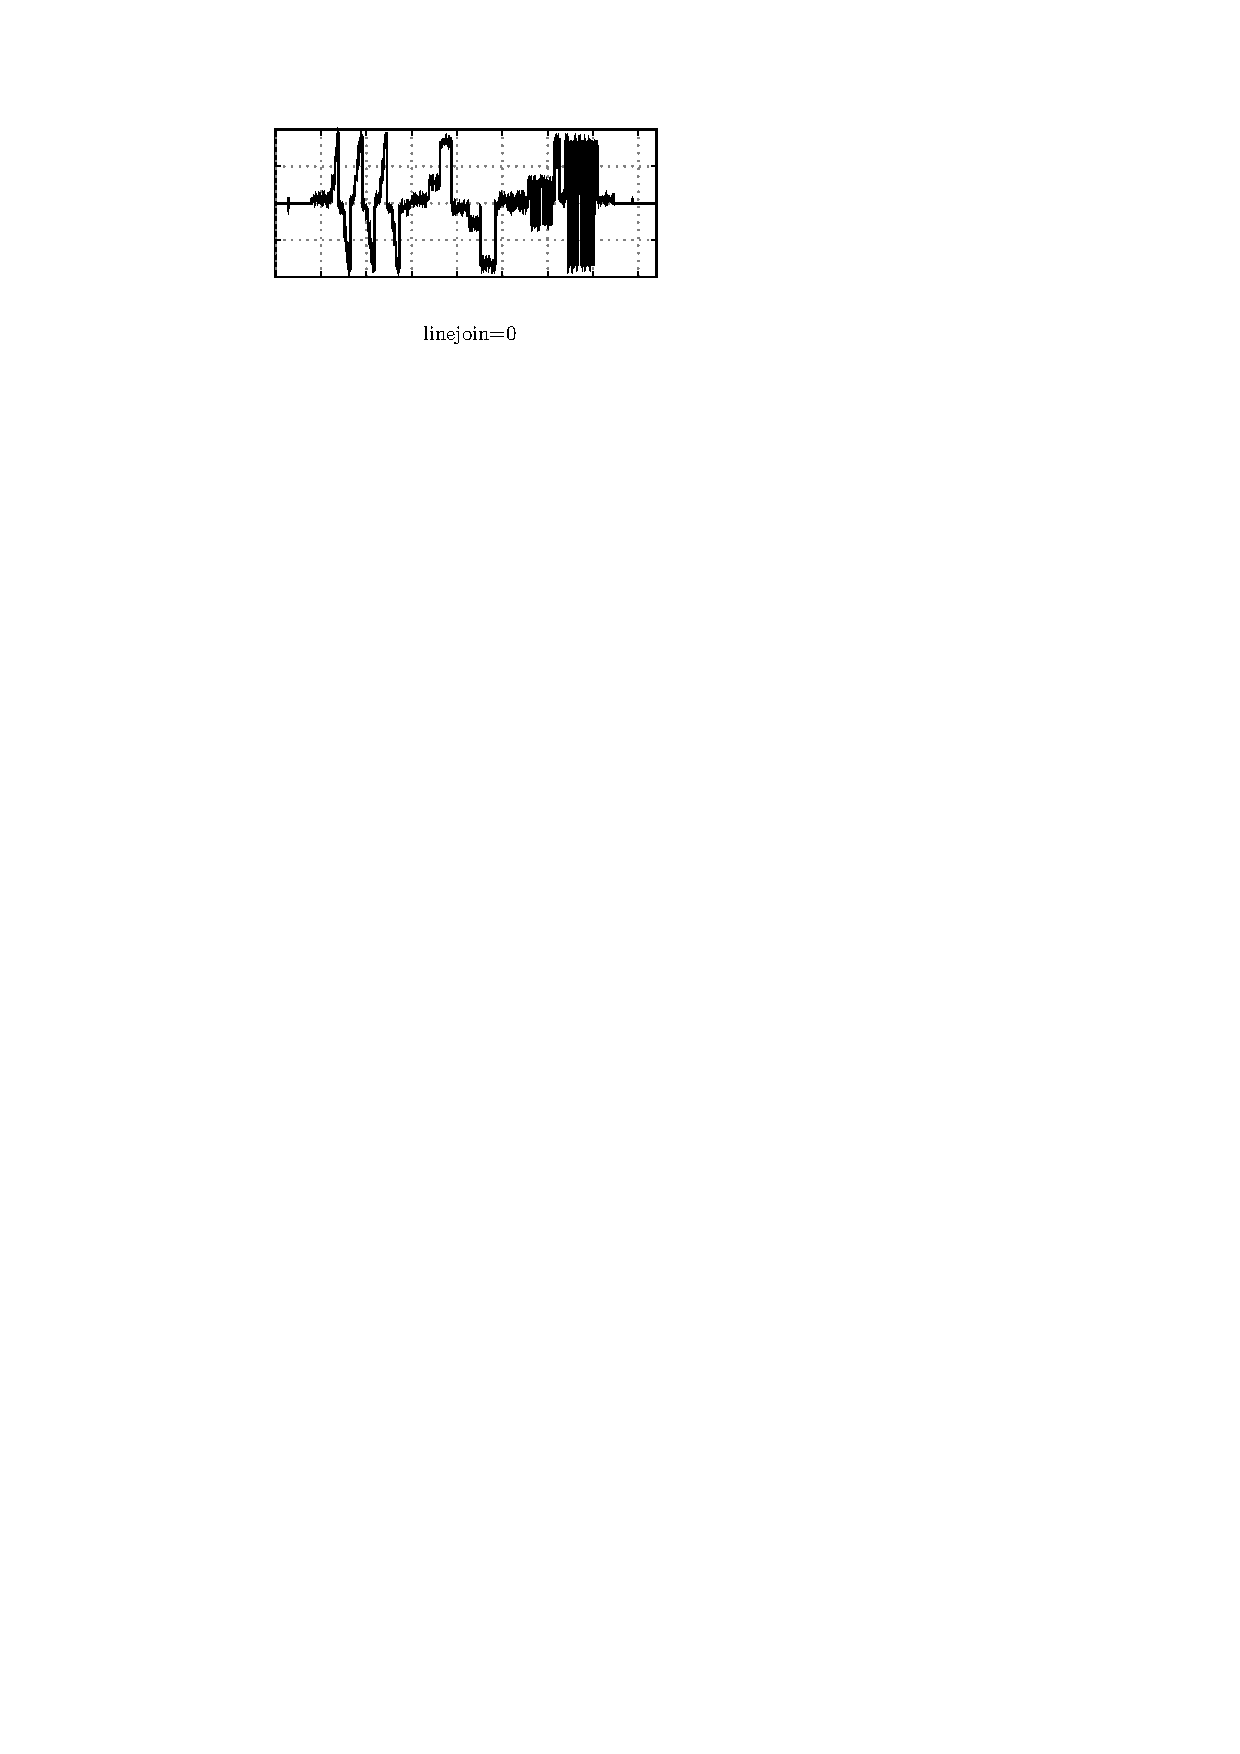
\includegraphics{fig_NoiseData_ClosedLine}
\end{minipage}
\begin{minipage}{0.48\linewidth}
	\centering
	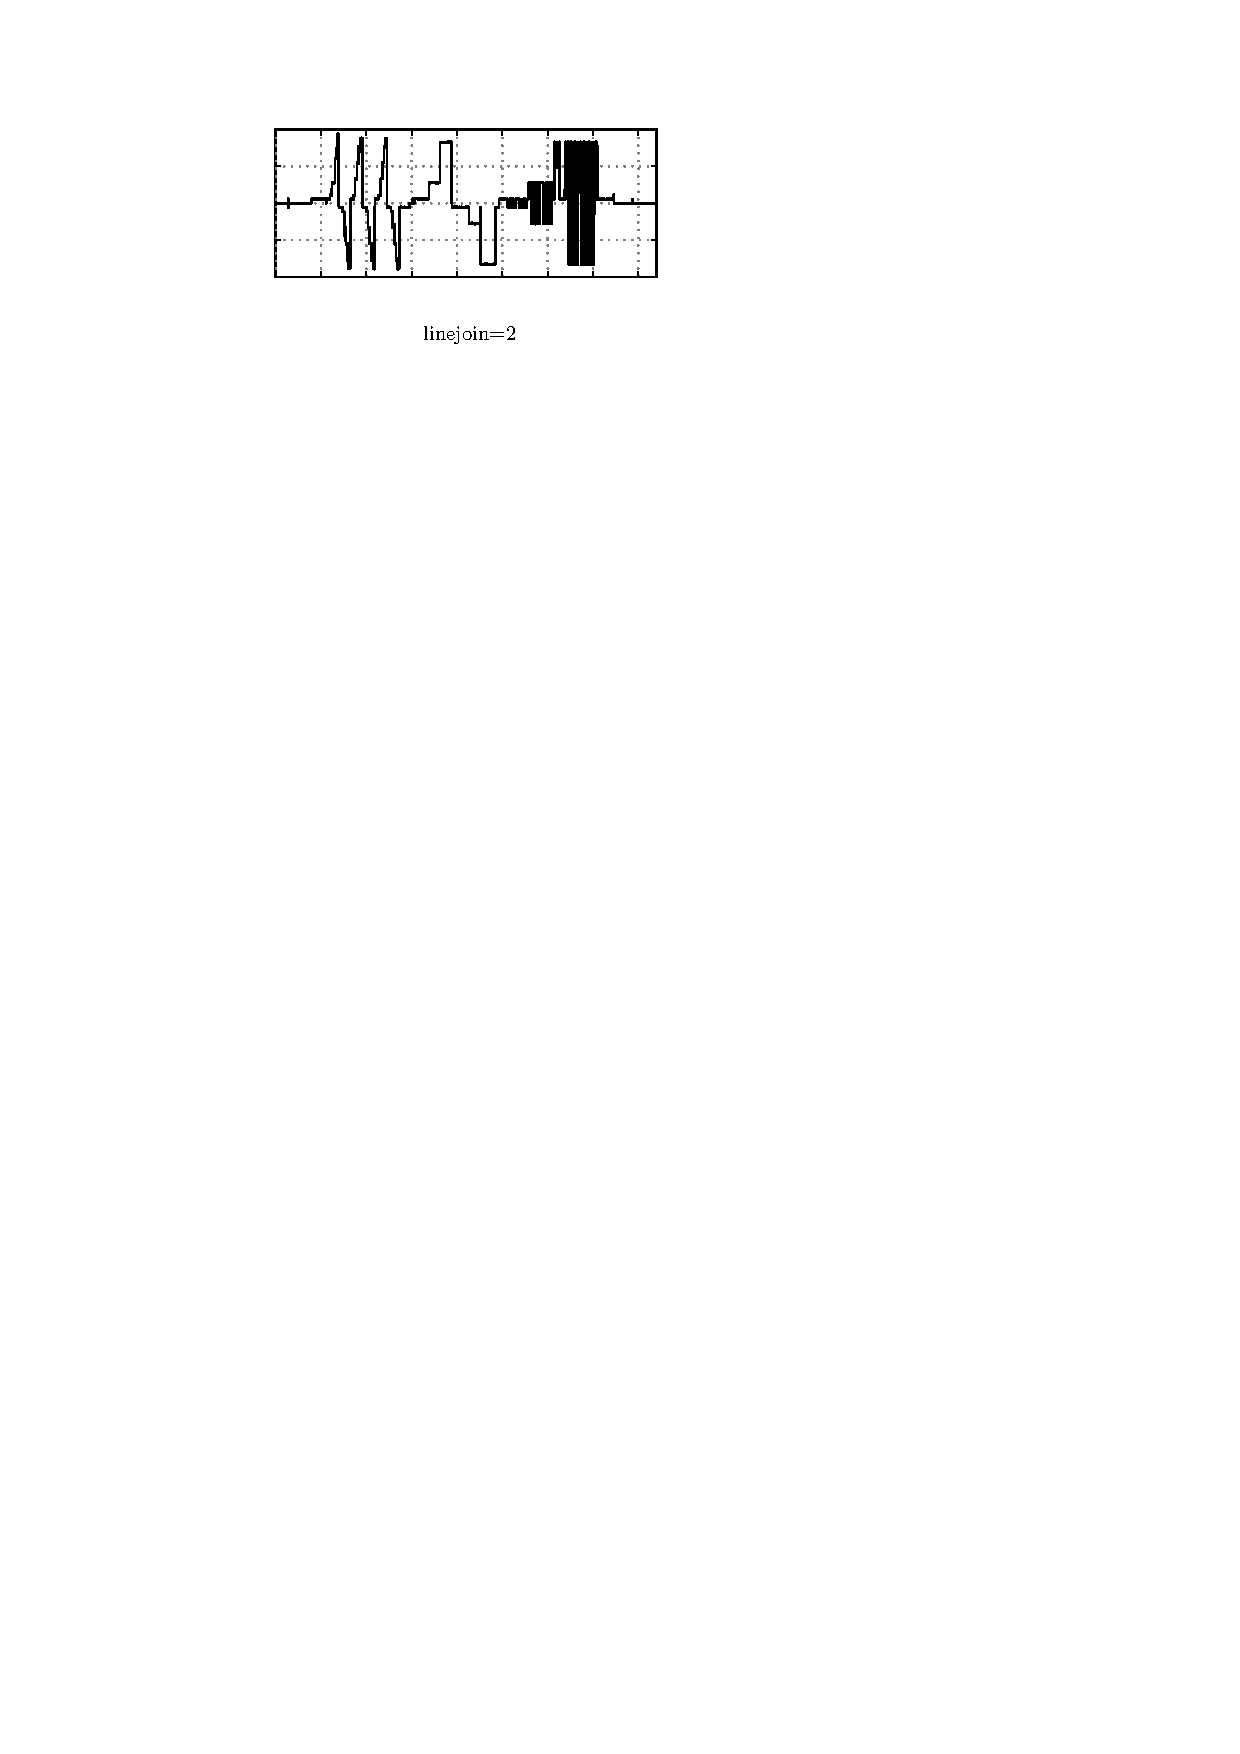
\includegraphics{fig_NoiseData_OpenLine}
\end{minipage}



\subsection{Customized Tick Labels}\label{sec:CustomTickLabels}

A common task is to plot a graph without numeric tick labels but with selected customized labels. This is easily accomplished by setting the option \verb|NoTickLabel| when plotting the axis and adding the customized labels with the commands \verb|PutTickLabelXaxis| and \verb|PutTickLabelYaxis|. Note that when setting \verb|NoTickLabel| for an axis, the option \verb|ax| has to be set in each call of \verb|PutTickLabelXaxis| and \verb|PutTickLabelYaxis| according to the axis one wishes to place the label at. This is also required if only the lower x-axis or left y-axis are plotted and tick labelled.

\begin{minipage}[T]{0.5\linewidth}
	\lstinputlisting[linerange=5-12]{examples/furtherEx_TickLabels}
\end{minipage}
\hspace{1ex}
\begin{minipage}[T]{0.4\linewidth}
	\begin{NumericDataPlot}{\textwidth}{6cm}
	\setxAxis{xMin=1, xMax=1.6, Dx=0.1, DDx=0.2}
	\setyAxis{yMin=75, yMax=130, Dy=12.5}
	
	\plotxAxis[NoTickLabel]{x-axis label}
	\plotyAxis[NoLabel, NoTickLabel]{y-axis label}
	
	\PutTickLabelXaxis[x=1.2, ax=lower]{test}
	\PutTickLabelXaxis[x=1.1, ax=upper]{test1}

	\PutTickLabelYaxis[y=80, ax=left]{test}
	\PutTickLabelYaxis[y=100, ax=right]{test1}
	
	
	\listplot[style=StdLineStyA]{\IdentI}
	\listplot[style=StdLineStyB]{\IdentII}
	
\end{NumericDataPlot}
\end{minipage}


% Copyright 2010 Thomas Koenig, Alexander Michel
%
% This file is part of NumericPlots.
%
% NumericPlots is free software: you can redistribute it and/or modify
% it under the terms of the GNU General Public License as published by
% the Free Software Foundation, either version 3 of the License, or
% any later version.
%
% NumericPlots is distributed in the hope that it will be useful,
% but WITHOUT ANY WARRANTY; without even the implied warranty of
% MERCHANTABILITY or FITNESS FOR A PARTICULAR PURPOSE.  See the
% GNU General Public License for more details.
%
% You should have received a copy of the GNU General Public License
% along with NumericPlots.  If not, see <http://www.gnu.org/licenses/>.

\section{Some test plots}


% +++++++++++++++++++++++++++++++++++++++++++++++++++++++++++++++++
\subsection{example}

% EPLdata written by export2latex
% date: 04-Apr-2011

\def\ExpDate{04-Apr-2011}
\def\DataRadiusNewXmin{-2.40}
\def\DataRadiusNewXmax{2.40}
\def\DataRadiusNewYmin{545.57}
\def\DataRadiusNewYmax{545.75}
\def\DataRadiusNewDxV{0.96}
\def\DataRadiusNewDyV{0.03}
\def\DataRadiusNew{
-2.40000 545.74005
-2.30000 545.72656
-2.20000 545.71364
-2.10000 545.70130
-2.00000 545.68953
-1.90000 545.67834
-1.80000 545.66772
-1.70000 545.65768
-1.60000 545.64821
-1.50000 545.63932
-1.40000 545.63101
-1.30000 545.62327
-1.20000 545.61610
-1.10000 545.60951
-1.00000 545.60350
-0.90000 545.59806
-0.80000 545.59320
-0.70000 545.58891
-0.60000 545.58519
-0.50000 545.58206
-0.40000 545.57949
-0.30000 545.57751
-0.20000 545.57610
-0.10000 545.57526
0.00000 545.57500
0.10000 545.57531
0.20000 545.57620
0.30000 545.57767
0.40000 545.57971
0.50000 545.58233
0.60000 545.58552
0.70000 545.58928
0.80000 545.59363
0.90000 545.59854
1.00000 545.60404
1.10000 545.61010
1.20000 545.61675
1.30000 545.62397
1.40000 545.63176
1.50000 545.64013
1.60000 545.64907
1.70000 545.65859
1.80000 545.66869
1.90000 545.67936
2.00000 545.69061
2.10000 545.70243
2.20000 545.71482
2.30000 545.72780
2.40000 545.74134
}

\def\DataRMeasuredXmin{-1.0}
\def\DataRMeasuredXmax{1.0}
\def\DataRMeasuredYmin{-1.0}
\def\DataRMeasuredYmax{1.0}
\def\DataRMeasuredDxV{0.4}
\def\DataRMeasuredDyV{0.4}
\def\DataRMeasured{
0.00000 545.57500
0.00000 545.57500
}

\def\DataShapeMeasuredXmin{-1.76}
\def\DataShapeMeasuredXmax{1.76}
\def\DataShapeMeasuredYmin{-0.37}
\def\DataShapeMeasuredYmax{-0.26}
\def\DataShapeMeasuredDxV{0.70}
\def\DataShapeMeasuredDyV{0.02}
\def\DataShapeMeasured{
-1.76000 -0.27350
-1.75500 -0.27350
-1.75000 -0.27300
-1.74500 -0.27150
-1.74000 -0.27300
-1.73500 -0.27350
-1.73000 -0.27400
-1.72500 -0.27450
-1.72000 -0.27550
-1.71500 -0.27550
-1.71000 -0.27600
-1.70500 -0.27700
-1.70000 -0.27800
-1.69500 -0.27900
-1.69000 -0.28000
-1.68500 -0.28050
-1.68000 -0.28000
-1.67500 -0.28250
-1.67000 -0.28200
-1.66500 -0.28350
-1.66000 -0.28350
-1.65500 -0.28350
-1.65000 -0.28250
-1.64500 -0.28300
-1.64000 -0.28350
-1.63500 -0.28400
-1.63000 -0.28550
-1.62500 -0.28550
-1.62000 -0.28500
-1.61500 -0.28550
-1.61000 -0.28750
-1.60500 -0.28950
-1.60000 -0.28950
-1.59500 -0.28950
-1.59000 -0.29150
-1.58500 -0.29250
-1.58000 -0.29250
-1.57500 -0.29150
-1.57000 -0.29250
-1.56500 -0.29250
-1.56000 -0.29250
-1.55500 -0.29300
-1.55000 -0.29250
-1.54500 -0.29300
-1.54000 -0.29350
-1.53500 -0.29350
-1.53000 -0.29350
-1.52500 -0.29500
-1.52000 -0.29650
-1.51500 -0.29650
-1.51000 -0.29750
-1.50500 -0.29750
-1.50000 -0.29850
-1.49500 -0.29900
-1.49000 -0.29950
-1.48500 -0.29950
-1.48000 -0.30000
-1.47500 -0.30000
-1.47000 -0.30000
-1.46500 -0.30000
-1.46000 -0.30050
-1.45500 -0.30100
-1.45000 -0.30150
-1.44500 -0.30200
-1.44000 -0.30250
-1.43500 -0.30250
-1.43000 -0.30500
-1.42500 -0.30550
-1.42000 -0.30450
-1.41500 -0.30550
-1.41000 -0.30650
-1.40500 -0.30750
-1.40000 -0.30750
-1.39500 -0.30800
-1.39000 -0.30800
-1.38500 -0.30750
-1.38000 -0.30800
-1.37500 -0.30800
-1.37000 -0.30750
-1.36500 -0.30700
-1.36000 -0.30750
-1.35500 -0.30850
-1.35000 -0.30950
-1.34500 -0.31100
-1.34000 -0.31250
-1.33500 -0.31250
-1.33000 -0.31250
-1.32500 -0.31250
-1.32000 -0.31200
-1.31500 -0.31350
-1.31000 -0.31350
-1.30500 -0.31300
-1.30000 -0.31450
-1.29500 -0.31400
-1.29000 -0.31400
-1.28500 -0.31400
-1.28000 -0.31500
-1.27500 -0.31550
-1.27000 -0.31450
-1.26500 -0.31500
-1.26000 -0.31650
-1.25500 -0.31750
-1.25000 -0.31800
-1.24500 -0.31800
-1.24000 -0.31750
-1.23500 -0.31850
-1.23000 -0.32000
-1.22500 -0.31950
-1.22000 -0.31850
-1.21500 -0.31850
-1.21000 -0.32050
-1.20500 -0.31950
-1.20000 -0.32050
-1.19500 -0.32000
-1.19000 -0.32050
-1.18500 -0.32050
-1.18000 -0.32100
-1.17500 -0.32100
-1.17000 -0.32200
-1.16500 -0.32100
-1.16000 -0.32100
-1.15500 -0.32300
-1.15000 -0.32300
-1.14500 -0.32400
-1.14000 -0.32450
-1.13500 -0.32500
-1.13000 -0.32500
-1.12500 -0.32500
-1.12000 -0.32600
-1.11500 -0.32500
-1.11000 -0.32600
-1.10500 -0.32650
-1.10000 -0.32700
-1.09500 -0.32700
-1.09000 -0.32700
-1.08500 -0.32650
-1.08000 -0.32850
-1.07500 -0.32950
-1.07000 -0.32750
-1.06500 -0.32750
-1.06000 -0.32900
-1.05500 -0.33150
-1.05000 -0.33050
-1.04500 -0.33000
-1.04000 -0.32850
-1.03500 -0.32900
-1.03000 -0.33000
-1.02500 -0.32950
-1.02000 -0.33050
-1.01500 -0.33050
-1.01000 -0.33100
-1.00500 -0.33150
-1.00000 -0.33200
-0.99500 -0.33250
-0.99000 -0.33450
-0.98500 -0.33400
-0.98000 -0.33350
-0.97500 -0.33300
-0.97000 -0.33450
-0.96500 -0.33550
-0.96000 -0.33450
-0.95500 -0.33450
-0.95000 -0.33400
-0.94500 -0.33400
-0.94000 -0.33350
-0.93500 -0.33500
-0.93000 -0.33450
-0.92500 -0.33600
-0.92000 -0.33650
-0.91500 -0.33650
-0.91000 -0.33650
-0.90500 -0.33800
-0.90000 -0.33900
-0.89500 -0.33850
-0.89000 -0.33750
-0.88500 -0.33750
-0.88000 -0.33950
-0.87500 -0.33950
-0.87000 -0.33800
-0.86500 -0.33800
-0.86000 -0.33850
-0.85500 -0.33800
-0.85000 -0.33800
-0.84500 -0.33900
-0.84000 -0.33950
-0.83500 -0.34050
-0.83000 -0.34000
-0.82500 -0.34050
-0.82000 -0.34100
-0.81500 -0.34200
-0.81000 -0.34300
-0.80500 -0.34150
-0.80000 -0.34100
-0.79500 -0.34300
-0.79000 -0.34250
-0.78500 -0.34150
-0.78000 -0.34200
-0.77500 -0.34050
-0.77000 -0.34100
-0.76500 -0.34100
-0.76000 -0.34150
-0.75500 -0.34350
-0.75000 -0.34100
-0.74500 -0.34350
-0.74000 -0.34450
-0.73500 -0.34450
-0.73000 -0.34550
-0.72500 -0.34600
-0.72000 -0.34600
-0.71500 -0.34500
-0.71000 -0.34550
-0.70500 -0.34600
-0.70000 -0.34650
-0.69500 -0.34450
-0.69000 -0.34500
-0.68500 -0.34350
-0.68000 -0.34500
-0.67500 -0.34450
-0.67000 -0.34550
-0.66500 -0.34600
-0.66000 -0.34500
-0.65500 -0.34550
-0.65000 -0.34650
-0.64500 -0.34750
-0.64000 -0.34900
-0.63500 -0.34800
-0.63000 -0.34800
-0.62500 -0.34850
-0.62000 -0.34800
-0.61500 -0.35100
-0.61000 -0.34850
-0.60500 -0.34800
-0.60000 -0.34850
-0.59500 -0.34750
-0.59000 -0.34800
-0.58500 -0.34700
-0.58000 -0.34850
-0.57500 -0.34950
-0.57000 -0.34800
-0.56500 -0.34850
-0.56000 -0.35000
-0.55500 -0.35050
-0.55000 -0.35150
-0.54500 -0.35200
-0.54000 -0.35050
-0.53500 -0.35200
-0.53000 -0.35200
-0.52500 -0.35250
-0.52000 -0.35150
-0.51500 -0.35100
-0.51000 -0.35100
-0.50500 -0.35100
-0.50000 -0.35200
-0.49500 -0.35150
-0.49000 -0.35150
-0.48500 -0.35100
-0.48000 -0.35300
-0.47500 -0.35200
-0.47000 -0.35350
-0.46500 -0.35400
-0.46000 -0.35500
-0.45500 -0.35500
-0.45000 -0.35400
-0.44500 -0.35550
-0.44000 -0.35600
-0.43500 -0.35500
-0.43000 -0.35400
-0.42500 -0.35500
-0.42000 -0.35550
-0.41500 -0.35500
-0.41000 -0.35400
-0.40500 -0.35400
-0.40000 -0.35500
-0.39500 -0.35450
-0.39000 -0.35600
-0.38500 -0.35600
-0.38000 -0.35700
-0.37500 -0.35850
-0.37000 -0.35650
-0.36500 -0.35550
-0.36000 -0.35700
-0.35500 -0.35850
-0.35000 -0.35800
-0.34500 -0.35750
-0.34000 -0.35650
-0.33500 -0.35650
-0.33000 -0.35600
-0.32500 -0.35550
-0.32000 -0.35600
-0.31500 -0.35700
-0.31000 -0.35650
-0.30500 -0.35800
-0.30000 -0.35750
-0.29500 -0.35800
-0.29000 -0.35900
-0.28500 -0.36000
-0.28000 -0.35850
-0.27500 -0.35750
-0.27000 -0.35950
-0.26500 -0.36050
-0.26000 -0.36000
-0.25500 -0.35700
-0.25000 -0.35850
-0.24500 -0.35850
-0.24000 -0.35900
-0.23500 -0.35900
-0.23000 -0.35950
-0.22500 -0.35950
-0.22000 -0.35850
-0.21500 -0.35900
-0.21000 -0.35900
-0.20500 -0.36050
-0.20000 -0.36100
-0.19500 -0.36150
-0.19000 -0.35950
-0.18500 -0.35950
-0.18000 -0.36150
-0.17500 -0.36100
-0.17000 -0.36200
-0.16500 -0.35950
-0.16000 -0.36050
-0.15500 -0.36000
-0.15000 -0.36050
-0.14500 -0.36000
-0.14000 -0.36050
-0.13500 -0.36050
-0.13000 -0.35950
-0.12500 -0.36050
-0.12000 -0.36100
-0.11500 -0.36200
-0.11000 -0.36100
-0.10500 -0.36200
-0.10000 -0.36250
-0.09500 -0.36250
-0.09000 -0.36300
-0.08500 -0.36350
-0.08000 -0.36200
-0.07500 -0.36150
-0.07000 -0.36200
-0.06500 -0.36200
-0.06000 -0.36200
-0.05500 -0.36150
-0.05000 -0.36200
-0.04500 -0.36150
-0.04000 -0.36150
-0.03500 -0.36150
-0.03000 -0.36100
-0.02500 -0.36300
-0.02000 -0.36250
-0.01500 -0.36250
-0.01000 -0.36150
-0.00500 -0.36350
0.00000 -0.36400
0.00500 -0.36250
0.01000 -0.36250
0.01500 -0.36250
0.02000 -0.36250
0.02500 -0.36200
0.03000 -0.36250
0.03500 -0.36200
0.04000 -0.36150
0.04500 -0.36150
0.05000 -0.36100
0.05500 -0.36150
0.06000 -0.36250
0.06500 -0.36300
0.07000 -0.36200
0.07500 -0.36200
0.08000 -0.36250
0.08500 -0.36400
0.09000 -0.36250
0.09500 -0.36250
0.10000 -0.36150
0.10500 -0.36200
0.11000 -0.36150
0.11500 -0.36200
0.12000 -0.36050
0.12500 -0.36100
0.13000 -0.36150
0.13500 -0.36150
0.14000 -0.36100
0.14500 -0.36050
0.15000 -0.36200
0.15500 -0.36300
0.16000 -0.36150
0.16500 -0.36200
0.17000 -0.36200
0.17500 -0.36250
0.18000 -0.36150
0.18500 -0.36050
0.19000 -0.36050
0.19500 -0.36000
0.20000 -0.36000
0.20500 -0.35950
0.21000 -0.36000
0.21500 -0.36000
0.22000 -0.36100
0.22500 -0.36000
0.23000 -0.36000
0.23500 -0.36100
0.24000 -0.36000
0.24500 -0.36100
0.25000 -0.36050
0.25500 -0.36050
0.26000 -0.36000
0.26500 -0.36150
0.27000 -0.36000
0.27500 -0.36050
0.28000 -0.35900
0.28500 -0.35800
0.29000 -0.35850
0.29500 -0.35850
0.30000 -0.35800
0.30500 -0.35750
0.31000 -0.35850
0.31500 -0.35750
0.32000 -0.35900
0.32500 -0.35900
0.33000 -0.35900
0.33500 -0.35900
0.34000 -0.35900
0.34500 -0.35900
0.35000 -0.35900
0.35500 -0.35850
0.36000 -0.35750
0.36500 -0.35700
0.37000 -0.35750
0.37500 -0.35750
0.38000 -0.35750
0.38500 -0.35650
0.39000 -0.35650
0.39500 -0.35600
0.40000 -0.35600
0.40500 -0.35650
0.41000 -0.35700
0.41500 -0.35800
0.42000 -0.35650
0.42500 -0.35650
0.43000 -0.35600
0.43500 -0.35500
0.44000 -0.35600
0.44500 -0.35600
0.45000 -0.35550
0.45500 -0.35450
0.46000 -0.35450
0.46500 -0.35350
0.47000 -0.35300
0.47500 -0.35350
0.48000 -0.35250
0.48500 -0.35300
0.49000 -0.35350
0.49500 -0.35350
0.50000 -0.35400
0.50500 -0.35400
0.51000 -0.35250
0.51500 -0.35250
0.52000 -0.35350
0.52500 -0.35450
0.53000 -0.35350
0.53500 -0.35200
0.54000 -0.35200
0.54500 -0.35200
0.55000 -0.35100
0.55500 -0.35000
0.56000 -0.34950
0.56500 -0.35000
0.57000 -0.35050
0.57500 -0.34900
0.58000 -0.35000
0.58500 -0.35200
0.59000 -0.35150
0.59500 -0.35100
0.60000 -0.35050
0.60500 -0.35000
0.61000 -0.34950
0.61500 -0.35000
0.62000 -0.35000
0.62500 -0.34850
0.63000 -0.34900
0.63500 -0.34850
0.64000 -0.34800
0.64500 -0.34800
0.65000 -0.34700
0.65500 -0.34650
0.66000 -0.34650
0.66500 -0.34650
0.67000 -0.34800
0.67500 -0.34850
0.68000 -0.34850
0.68500 -0.34850
0.69000 -0.34700
0.69500 -0.34600
0.70000 -0.34650
0.70500 -0.34650
0.71000 -0.34600
0.71500 -0.34550
0.72000 -0.34400
0.72500 -0.34450
0.73000 -0.34400
0.73500 -0.34400
0.74000 -0.34400
0.74500 -0.34400
0.75000 -0.34400
0.75500 -0.34400
0.76000 -0.34250
0.76500 -0.34450
0.77000 -0.34400
0.77500 -0.34400
0.78000 -0.34400
0.78500 -0.34300
0.79000 -0.34200
0.79500 -0.34300
0.80000 -0.34150
0.80500 -0.34150
0.81000 -0.34100
0.81500 -0.33900
0.82000 -0.34050
0.82500 -0.34050
0.83000 -0.34000
0.83500 -0.34000
0.84000 -0.34000
0.84500 -0.33850
0.85000 -0.34050
0.85500 -0.34050
0.86000 -0.34000
0.86500 -0.34000
0.87000 -0.34100
0.87500 -0.33850
0.88000 -0.33950
0.88500 -0.33850
0.89000 -0.33700
0.89500 -0.33700
0.90000 -0.33750
0.90500 -0.33650
0.91000 -0.33600
0.91500 -0.33650
0.92000 -0.33550
0.92500 -0.33500
0.93000 -0.33500
0.93500 -0.33450
0.94000 -0.33550
0.94500 -0.33450
0.95000 -0.33450
0.95500 -0.33450
0.96000 -0.33600
0.96500 -0.33450
0.97000 -0.33450
0.97500 -0.33450
0.98000 -0.33400
0.98500 -0.33350
0.99000 -0.33250
0.99500 -0.33200
1.00000 -0.33250
1.00500 -0.33150
1.01000 -0.33100
1.01500 -0.33100
1.02000 -0.33000
1.02500 -0.33200
1.03000 -0.33150
1.03500 -0.33200
1.04000 -0.33200
1.04500 -0.33150
1.05000 -0.33050
1.05500 -0.33000
1.06000 -0.33100
1.06500 -0.33000
1.07000 -0.32850
1.07500 -0.32800
1.08000 -0.32800
1.08500 -0.32700
1.09000 -0.32700
1.09500 -0.32600
1.10000 -0.32650
1.10500 -0.32600
1.11000 -0.32650
1.11500 -0.32650
1.12000 -0.32600
1.12500 -0.32500
1.13000 -0.32600
1.13500 -0.32700
1.14000 -0.32550
1.14500 -0.32550
1.15000 -0.32550
1.15500 -0.32450
1.16000 -0.32300
1.16500 -0.32250
1.17000 -0.32250
1.17500 -0.32200
1.18000 -0.32100
1.18500 -0.32100
1.19000 -0.32050
1.19500 -0.32100
1.20000 -0.32150
1.20500 -0.32100
1.21000 -0.32050
1.21500 -0.32150
1.22000 -0.32100
1.22500 -0.32100
1.23000 -0.31950
1.23500 -0.32000
1.24000 -0.31950
1.24500 -0.31950
1.25000 -0.31800
1.25500 -0.31800
1.26000 -0.31650
1.26500 -0.31550
1.27000 -0.31550
1.27500 -0.31550
1.28000 -0.31500
1.28500 -0.31500
1.29000 -0.31450
1.29500 -0.31450
1.30000 -0.31500
1.30500 -0.31500
1.31000 -0.31450
1.31500 -0.31400
1.32000 -0.31350
1.32500 -0.31200
1.33000 -0.31150
1.33500 -0.31250
1.34000 -0.31050
1.34500 -0.31050
1.35000 -0.31000
1.35500 -0.30950
1.36000 -0.30950
1.36500 -0.30850
1.37000 -0.30850
1.37500 -0.30800
1.38000 -0.30750
1.38500 -0.30700
1.39000 -0.30750
1.39500 -0.30700
1.40000 -0.30500
1.40500 -0.30550
1.41000 -0.30550
1.41500 -0.30600
1.42000 -0.30500
1.42500 -0.30350
1.43000 -0.30350
1.43500 -0.30250
1.44000 -0.30150
1.44500 -0.30250
1.45000 -0.30150
1.45500 -0.30200
1.46000 -0.30000
1.46500 -0.29950
1.47000 -0.30000
1.47500 -0.29900
1.48000 -0.30000
1.48500 -0.29900
1.49000 -0.29750
1.49500 -0.29650
1.50000 -0.29650
1.50500 -0.29650
1.51000 -0.29500
1.51500 -0.29400
1.52000 -0.29450
1.52500 -0.29350
1.53000 -0.29300
1.53500 -0.29300
1.54000 -0.29250
1.54500 -0.29300
1.55000 -0.29300
1.55500 -0.29100
1.56000 -0.28950
1.56500 -0.29000
1.57000 -0.29000
1.57500 -0.28950
1.58000 -0.28800
1.58500 -0.28700
1.59000 -0.28750
1.59500 -0.28700
1.60000 -0.28550
1.60500 -0.28400
1.61000 -0.28350
1.61500 -0.28450
1.62000 -0.28400
1.62500 -0.28300
1.63000 -0.28300
1.63500 -0.28200
1.64000 -0.28100
1.64500 -0.28050
1.65000 -0.28050
1.65500 -0.28000
1.66000 -0.27900
1.66500 -0.27800
1.67000 -0.27700
1.67500 -0.27600
1.68000 -0.27650
1.68500 -0.27500
1.69000 -0.27350
1.69500 -0.27350
1.70000 -0.27350
1.70500 -0.27150
1.71000 -0.27100
1.71500 -0.27100
1.72000 -0.27050
1.72500 -0.27000
1.73000 -0.27000
1.73500 -0.26850
1.74000 -0.26850
1.74500 -0.26850
1.75000 -0.26700
1.75500 -0.26450
1.76000 -0.26450
}

\def\DataShapeFittedXmin{-2.40}
\def\DataShapeFittedXmax{2.40}
\def\DataShapeFittedYmin{-0.37}
\def\DataShapeFittedYmax{-0.19}
\def\DataShapeFittedDxV{0.96}
\def\DataShapeFittedDyV{0.03}
\def\DataShapeFitted{
-2.40000 -0.19595
-2.30000 -0.20945
-2.20000 -0.22237
-2.10000 -0.23471
-2.00000 -0.24648
-1.90000 -0.25767
-1.80000 -0.26828
-1.70000 -0.27833
-1.60000 -0.28779
-1.50000 -0.29668
-1.40000 -0.30500
-1.30000 -0.31274
-1.20000 -0.31990
-1.10000 -0.32649
-1.00000 -0.33251
-0.90000 -0.33795
-0.80000 -0.34281
-0.70000 -0.34710
-0.60000 -0.35081
-0.50000 -0.35395
-0.40000 -0.35651
-0.30000 -0.35850
-0.20000 -0.35991
-0.10000 -0.36074
0.00000 -0.36100
0.10000 -0.36069
0.20000 -0.35980
0.30000 -0.35833
0.40000 -0.35629
0.50000 -0.35368
0.60000 -0.35049
0.70000 -0.34672
0.80000 -0.34238
0.90000 -0.33746
1.00000 -0.33197
1.10000 -0.32590
1.20000 -0.31926
1.30000 -0.31204
1.40000 -0.30424
1.50000 -0.29587
1.60000 -0.28693
1.70000 -0.27741
1.80000 -0.26732
1.90000 -0.25664
2.00000 -0.24540
2.10000 -0.23358
2.20000 -0.22118
2.30000 -0.20821
2.40000 -0.19466
}

\def\DataRadiusXmin{-2.40}
\def\DataRadiusXmax{2.40}
\def\DataRadiusYmin{545.29}
\def\DataRadiusYmax{545.75}
\def\DataRadiusDxV{0.96}
\def\DataRadiusDyV{0.09}
\def\DataRadius{
-2.40000 545.74005
-2.30000 545.72656
-2.20000 545.71364
-2.10000 545.70130
-2.00000 545.68953
-1.90000 545.67834
-1.80000 545.55480
-1.70000 545.47646
-1.60000 545.45875
-1.50000 545.44509
-1.40000 545.43527
-1.30000 545.42238
-1.20000 545.37810
-1.10000 545.35977
-1.00000 545.34183
-0.90000 545.33194
-0.80000 545.31895
-0.70000 545.31302
-0.60000 545.30891
-0.50000 545.30577
-0.40000 545.30321
-0.30000 545.30123
-0.20000 545.29981
-0.10000 545.29898
0.00000 545.29872
0.10000 545.29903
0.20000 545.29992
0.30000 545.30139
0.40000 545.30343
0.50000 545.30604
0.60000 545.30924
0.70000 545.31340
0.80000 545.31938
0.90000 545.33243
1.00000 545.34236
1.10000 545.36036
1.20000 545.37874
1.30000 545.42308
1.40000 545.43602
1.50000 545.44589
1.60000 545.45961
1.70000 545.47737
1.80000 545.55576
1.90000 545.67936
2.00000 545.69061
2.10000 545.70243
2.20000 545.71482
2.30000 545.72780
2.40000 545.74134
}

\def\DataWearXmin{-2.40}
\def\DataWearXmax{2.40}
\def\DataWearYmin{-0.28}
\def\DataWearYmax{0.00}
\def\DataWearDxV{0.96}
\def\DataWearDyV{0.06}
\def\DataWear{
-2.40000 0.00000
-2.30000 0.00000
-2.20000 0.00000
-2.10000 0.00000
-2.00000 0.00000
-1.90000 0.00000
-1.80000 -0.11292
-1.70000 -0.18122
-1.60000 -0.18946
-1.50000 -0.19423
-1.40000 -0.19574
-1.30000 -0.20088
-1.20000 -0.23800
-1.10000 -0.24974
-1.00000 -0.26167
-0.90000 -0.26612
-0.80000 -0.27425
-0.70000 -0.27589
-0.60000 -0.27628
-0.50000 -0.27628
-0.40000 -0.27628
-0.30000 -0.27628
-0.20000 -0.27628
-0.10000 -0.27628
0.00000 -0.27628
0.10000 -0.27628
0.20000 -0.27628
0.30000 -0.27628
0.40000 -0.27628
0.50000 -0.27628
0.60000 -0.27628
0.70000 -0.27589
0.80000 -0.27425
0.90000 -0.26612
1.00000 -0.26167
1.10000 -0.24974
1.20000 -0.23800
1.30000 -0.20088
1.40000 -0.19574
1.50000 -0.19423
1.60000 -0.18946
1.70000 -0.18122
1.80000 -0.11292
1.90000 0.00000
2.00000 0.00000
2.10000 0.00000
2.20000 0.00000
2.30000 0.00000
2.40000 0.00000
}

\def\DataRadiusUsedXmin{-1.77}
\def\DataRadiusUsedXmax{1.77}
\def\DataRadiusUsedYmin{545.21}
\def\DataRadiusUsedYmax{545.50}
\def\DataRadiusUsedDxV{0.71}
\def\DataRadiusUsedDyV{0.06}
\def\DataRadiusUsed{
-1.77000 545.48417
-1.76500 545.48317
-1.76000 545.48317
-1.75500 545.48267
-1.75000 545.48117
-1.74500 545.47967
-1.74000 545.47717
-1.73500 545.47617
-1.73000 545.47417
-1.72500 545.47167
-1.72000 545.47067
-1.71500 545.46867
-1.71000 545.46767
-1.70500 545.46717
-1.70000 545.46667
-1.69500 545.46567
-1.69000 545.46367
-1.68500 545.46267
-1.68000 545.46267
-1.67500 545.46067
-1.67000 545.45917
-1.66500 545.45717
-1.66000 545.45617
-1.65500 545.45367
-1.65000 545.45167
-1.64500 545.44867
-1.64000 545.44767
-1.63500 545.44517
-1.63000 545.44217
-1.62500 545.43917
-1.62000 545.43717
-1.61500 545.43317
-1.61000 545.42967
-1.60500 545.42517
-1.60000 545.42117
-1.59500 545.41667
-1.59000 545.41217
-1.58500 545.40767
-1.58000 545.40367
-1.57500 545.40017
-1.57000 545.39717
-1.56500 545.39467
-1.56000 545.39117
-1.55500 545.38767
-1.55000 545.38617
-1.54500 545.38317
-1.54000 545.38117
-1.53500 545.38117
-1.53000 545.37917
-1.52500 545.37817
-1.52000 545.37517
-1.51500 545.37367
-1.51000 545.37217
-1.50500 545.36967
-1.50000 545.36917
-1.49500 545.36817
-1.49000 545.36567
-1.48500 545.36517
-1.48000 545.36267
-1.47500 545.36267
-1.47000 545.36017
-1.46500 545.35917
-1.46000 545.35917
-1.45500 545.35667
-1.45000 545.35567
-1.44500 545.35567
-1.44000 545.35417
-1.43500 545.35517
-1.43000 545.35417
-1.42500 545.35167
-1.42000 545.35117
-1.41500 545.34967
-1.41000 545.34867
-1.40500 545.34867
-1.40000 545.34817
-1.39500 545.34567
-1.39000 545.34567
-1.38500 545.34367
-1.38000 545.34267
-1.37500 545.34217
-1.37000 545.34217
-1.36500 545.34017
-1.36000 545.33817
-1.35500 545.33717
-1.35000 545.33467
-1.34500 545.33167
-1.34000 545.32867
-1.33500 545.32667
-1.33000 545.32517
-1.32500 545.32167
-1.32000 545.31917
-1.31500 545.31667
-1.31000 545.31567
-1.30500 545.31067
-1.30000 545.30867
-1.29500 545.30567
-1.29000 545.30367
-1.28500 545.30267
-1.28000 545.29817
-1.27500 545.29467
-1.27000 545.29267
-1.26500 545.29217
-1.26000 545.29117
-1.25500 545.29017
-1.25000 545.28817
-1.24500 545.28817
-1.24000 545.28567
-1.23500 545.28367
-1.23000 545.28317
-1.22500 545.28267
-1.22000 545.28117
-1.21500 545.27867
-1.21000 545.27617
-1.20500 545.27667
-1.20000 545.27567
-1.19500 545.27267
-1.19000 545.27117
-1.18500 545.27117
-1.18000 545.27067
-1.17500 545.27067
-1.17000 545.27017
-1.16500 545.26867
-1.16000 545.26817
-1.15500 545.26717
-1.15000 545.26867
-1.14500 545.26867
-1.14000 545.26567
-1.13500 545.26417
-1.13000 545.26417
-1.12500 545.26217
-1.12000 545.26267
-1.11500 545.26117
-1.11000 545.26067
-1.10500 545.26017
-1.10000 545.25867
-1.09500 545.25717
-1.09000 545.25717
-1.08500 545.25767
-1.08000 545.25617
-1.07500 545.25517
-1.07000 545.25417
-1.06500 545.25367
-1.06000 545.25517
-1.05500 545.25517
-1.05000 545.25217
-1.04500 545.25017
-1.04000 545.24867
-1.03500 545.24917
-1.03000 545.24717
-1.02500 545.24667
-1.02000 545.24617
-1.01500 545.24267
-1.01000 545.24217
-1.00500 545.24017
-1.00000 545.23917
-0.99500 545.23817
-0.99000 545.23667
-0.98500 545.23617
-0.98000 545.23717
-0.97500 545.23617
-0.97000 545.23817
-0.96500 545.23617
-0.96000 545.23617
-0.95500 545.23467
-0.95000 545.23167
-0.94500 545.23067
-0.94000 545.23017
-0.93500 545.23067
-0.93000 545.23167
-0.92500 545.23067
-0.92000 545.23167
-0.91500 545.23067
-0.91000 545.23017
-0.90500 545.22967
-0.90000 545.22917
-0.89500 545.22917
-0.89000 545.23017
-0.88500 545.22867
-0.88000 545.22867
-0.87500 545.22817
-0.87000 545.22767
-0.86500 545.22917
-0.86000 545.22867
-0.85500 545.22867
-0.85000 545.22817
-0.84500 545.22767
-0.84000 545.22917
-0.83500 545.22717
-0.83000 545.22817
-0.82500 545.22717
-0.82000 545.22617
-0.81500 545.22667
-0.81000 545.22717
-0.80500 545.22667
-0.80000 545.22717
-0.79500 545.22867
-0.79000 545.22717
-0.78500 545.22367
-0.78000 545.22217
-0.77500 545.22167
-0.77000 545.22267
-0.76500 545.22467
-0.76000 545.22717
-0.75500 545.22767
-0.75000 545.22817
-0.74500 545.22967
-0.74000 545.22967
-0.73500 545.22917
-0.73000 545.23017
-0.72500 545.22917
-0.72000 545.22717
-0.71500 545.22617
-0.71000 545.22667
-0.70500 545.22667
-0.70000 545.22817
-0.69500 545.22667
-0.69000 545.22617
-0.68500 545.22667
-0.68000 545.22667
-0.67500 545.22817
-0.67000 545.22567
-0.66500 545.22567
-0.66000 545.22717
-0.65500 545.22767
-0.65000 545.22617
-0.64500 545.22667
-0.64000 545.22617
-0.63500 545.22617
-0.63000 545.22617
-0.62500 545.22467
-0.62000 545.22517
-0.61500 545.22567
-0.61000 545.22667
-0.60500 545.22667
-0.60000 545.22517
-0.59500 545.22617
-0.59000 545.22817
-0.58500 545.22967
-0.58000 545.23067
-0.57500 545.22867
-0.57000 545.22817
-0.56500 545.22817
-0.56000 545.22817
-0.55500 545.22767
-0.55000 545.22767
-0.54500 545.22967
-0.54000 545.22967
-0.53500 545.22967
-0.53000 545.22917
-0.52500 545.23017
-0.52000 545.23117
-0.51500 545.23017
-0.51000 545.23017
-0.50500 545.22917
-0.50000 545.22867
-0.49500 545.22917
-0.49000 545.22917
-0.48500 545.22917
-0.48000 545.22917
-0.47500 545.23017
-0.47000 545.22917
-0.46500 545.22967
-0.46000 545.22917
-0.45500 545.22817
-0.45000 545.22867
-0.44500 545.22767
-0.44000 545.22767
-0.43500 545.22567
-0.43000 545.22517
-0.42500 545.22617
-0.42000 545.22767
-0.41500 545.23067
-0.41000 545.23017
-0.40500 545.22867
-0.40000 545.22867
-0.39500 545.22767
-0.39000 545.22817
-0.38500 545.22817
-0.38000 545.22717
-0.37500 545.22567
-0.37000 545.22417
-0.36500 545.22367
-0.36000 545.22367
-0.35500 545.22617
-0.35000 545.22667
-0.34500 545.22617
-0.34000 545.22617
-0.33500 545.22517
-0.33000 545.22367
-0.32500 545.22417
-0.32000 545.22417
-0.31500 545.22367
-0.31000 545.22417
-0.30500 545.22367
-0.30000 545.22417
-0.29500 545.22517
-0.29000 545.22317
-0.28500 545.22267
-0.28000 545.22517
-0.27500 545.22467
-0.27000 545.22667
-0.26500 545.22517
-0.26000 545.22467
-0.25500 545.22317
-0.25000 545.22217
-0.24500 545.22167
-0.24000 545.22367
-0.23500 545.22517
-0.23000 545.22517
-0.22500 545.22267
-0.22000 545.22117
-0.21500 545.22117
-0.21000 545.22267
-0.20500 545.22467
-0.20000 545.22617
-0.19500 545.22667
-0.19000 545.22667
-0.18500 545.22817
-0.18000 545.22817
-0.17500 545.22717
-0.17000 545.22617
-0.16500 545.22517
-0.16000 545.22417
-0.15500 545.22417
-0.15000 545.22317
-0.14500 545.22467
-0.14000 545.22317
-0.13500 545.22117
-0.13000 545.22167
-0.12500 545.22417
-0.12000 545.22217
-0.11500 545.22217
-0.11000 545.22167
-0.10500 545.22167
-0.10000 545.21967
-0.09500 545.21967
-0.09000 545.21917
-0.08500 545.21967
-0.08000 545.21817
-0.07500 545.21917
-0.07000 545.21967
-0.06500 545.22067
-0.06000 545.22067
-0.05500 545.22117
-0.05000 545.22367
-0.04500 545.22367
-0.04000 545.22317
-0.03500 545.22317
-0.03000 545.22417
-0.02500 545.22317
-0.02000 545.22317
-0.01500 545.22167
-0.01000 545.22167
-0.00500 545.22017
0.00000 545.22017
0.00500 545.21967
0.01000 545.22067
0.01500 545.21967
0.02000 545.21967
0.02500 545.22117
0.03000 545.21917
0.03500 545.21867
0.04000 545.21867
0.04500 545.22017
0.05000 545.22017
0.05500 545.22167
0.06000 545.22067
0.06500 545.22017
0.07000 545.21967
0.07500 545.21967
0.08000 545.22067
0.08500 545.22117
0.09000 545.22067
0.09500 545.22217
0.10000 545.22067
0.10500 545.21817
0.11000 545.21917
0.11500 545.21867
0.12000 545.21867
0.12500 545.21717
0.13000 545.21867
0.13500 545.21917
0.14000 545.22067
0.14500 545.22267
0.15000 545.22367
0.15500 545.22417
0.16000 545.22267
0.16500 545.22217
0.17000 545.22367
0.17500 545.22267
0.18000 545.22517
0.18500 545.22717
0.19000 545.22617
0.19500 545.22717
0.20000 545.22667
0.20500 545.22717
0.21000 545.22667
0.21500 545.22717
0.22000 545.22767
0.22500 545.22667
0.23000 545.22617
0.23500 545.22667
0.24000 545.22467
0.24500 545.22367
0.25000 545.22417
0.25500 545.22317
0.26000 545.22417
0.26500 545.22367
0.27000 545.22467
0.27500 545.22267
0.28000 545.22317
0.28500 545.22217
0.29000 545.22467
0.29500 545.22717
0.30000 545.22717
0.30500 545.22817
0.31000 545.22717
0.31500 545.22767
0.32000 545.22767
0.32500 545.22817
0.33000 545.22817
0.33500 545.22717
0.34000 545.22717
0.34500 545.22667
0.35000 545.22817
0.35500 545.22667
0.36000 545.22617
0.36500 545.22717
0.37000 545.22617
0.37500 545.22767
0.38000 545.22867
0.38500 545.22767
0.39000 545.22817
0.39500 545.22867
0.40000 545.22867
0.40500 545.22967
0.41000 545.22817
0.41500 545.22867
0.42000 545.22867
0.42500 545.22967
0.43000 545.22867
0.43500 545.22867
0.44000 545.23017
0.44500 545.22817
0.45000 545.22667
0.45500 545.22517
0.46000 545.22667
0.46500 545.22767
0.47000 545.22817
0.47500 545.22917
0.48000 545.22967
0.48500 545.22967
0.49000 545.22917
0.49500 545.22817
0.50000 545.23017
0.50500 545.23217
0.51000 545.23067
0.51500 545.23017
0.52000 545.23067
0.52500 545.22967
0.53000 545.22867
0.53500 545.22867
0.54000 545.22867
0.54500 545.22867
0.55000 545.22617
0.55500 545.22467
0.56000 545.22367
0.56500 545.22217
0.57000 545.22217
0.57500 545.22167
0.58000 545.22317
0.58500 545.22417
0.59000 545.22567
0.59500 545.22567
0.60000 545.22517
0.60500 545.22517
0.61000 545.22467
0.61500 545.22317
0.62000 545.22367
0.62500 545.22417
0.63000 545.22417
0.63500 545.22367
0.64000 545.22117
0.64500 545.22067
0.65000 545.22067
0.65500 545.22017
0.66000 545.22067
0.66500 545.21917
0.67000 545.21867
0.67500 545.21817
0.68000 545.21667
0.68500 545.21717
0.69000 545.21617
0.69500 545.21417
0.70000 545.21267
0.70500 545.21317
0.71000 545.21267
0.71500 545.21267
0.72000 545.21517
0.72500 545.21717
0.73000 545.21767
0.73500 545.21967
0.74000 545.22317
0.74500 545.22467
0.75000 545.22717
0.75500 545.22717
0.76000 545.22767
0.76500 545.22867
0.77000 545.22967
0.77500 545.23117
0.78000 545.23467
0.78500 545.23667
0.79000 545.23917
0.79500 545.24167
0.80000 545.24267
0.80500 545.24267
0.81000 545.24267
0.81500 545.24317
0.82000 545.24317
0.82500 545.24417
0.83000 545.24567
0.83500 545.24467
0.84000 545.24567
0.84500 545.24517
0.85000 545.24517
0.85500 545.24517
0.86000 545.24667
0.86500 545.24617
0.87000 545.24617
0.87500 545.24667
0.88000 545.24667
0.88500 545.24617
0.89000 545.24567
0.89500 545.24767
0.90000 545.24717
0.90500 545.24567
0.91000 545.24617
0.91500 545.24717
0.92000 545.24717
0.92500 545.24967
0.93000 545.25117
0.93500 545.25117
0.94000 545.25117
0.94500 545.25067
0.95000 545.25167
0.95500 545.25117
0.96000 545.25317
0.96500 545.25317
0.97000 545.25517
0.97500 545.25667
0.98000 545.25517
0.98500 545.25667
0.99000 545.25667
0.99500 545.25817
1.00000 545.25917
1.00500 545.25917
1.01000 545.26017
1.01500 545.26217
1.02000 545.26367
1.02500 545.26367
1.03000 545.26417
1.03500 545.26417
1.04000 545.26467
1.04500 545.26617
1.05000 545.26667
1.05500 545.26567
1.06000 545.26667
1.06500 545.26517
1.07000 545.26217
1.07500 545.26217
1.08000 545.26067
1.08500 545.26217
1.09000 545.26317
1.09500 545.26367
1.10000 545.26317
1.10500 545.26267
1.11000 545.26267
1.11500 545.26417
1.12000 545.26517
1.12500 545.26717
1.13000 545.27017
1.13500 545.27317
1.14000 545.27467
1.14500 545.27717
1.15000 545.27717
1.15500 545.27917
1.16000 545.28017
1.16500 545.27867
1.17000 545.28067
1.17500 545.28117
1.18000 545.28317
1.18500 545.28267
1.19000 545.28117
1.19500 545.27967
1.20000 545.28017
1.20500 545.27867
1.21000 545.28017
1.21500 545.28217
1.22000 545.28517
1.22500 545.28667
1.23000 545.28617
1.23500 545.28617
1.24000 545.28717
1.24500 545.28967
1.25000 545.29317
1.25500 545.29167
1.26000 545.29317
1.26500 545.29367
1.27000 545.29617
1.27500 545.29817
1.28000 545.30117
1.28500 545.30317
1.29000 545.30617
1.29500 545.30617
1.30000 545.30867
1.30500 545.31217
1.31000 545.31617
1.31500 545.31917
1.32000 545.32217
1.32500 545.32267
1.33000 545.32617
1.33500 545.32767
1.34000 545.33117
1.34500 545.33467
1.35000 545.33617
1.35500 545.33867
1.36000 545.33917
1.36500 545.34067
1.37000 545.34267
1.37500 545.34567
1.38000 545.34717
1.38500 545.34867
1.39000 545.34967
1.39500 545.35217
1.40000 545.35317
1.40500 545.35317
1.41000 545.35367
1.41500 545.35467
1.42000 545.35667
1.42500 545.35767
1.43000 545.35917
1.43500 545.35867
1.44000 545.35917
1.44500 545.35917
1.45000 545.35967
1.45500 545.36067
1.46000 545.36167
1.46500 545.36167
1.47000 545.36417
1.47500 545.36467
1.48000 545.36317
1.48500 545.36217
1.49000 545.36067
1.49500 545.36067
1.50000 545.36217
1.50500 545.36567
1.51000 545.36817
1.51500 545.37117
1.52000 545.37217
1.52500 545.37367
1.53000 545.37217
1.53500 545.37017
1.54000 545.37117
1.54500 545.37367
1.55000 545.37867
1.55500 545.38617
1.56000 545.39317
1.56500 545.39717
1.57000 545.40017
1.57500 545.40367
1.58000 545.40867
1.58500 545.41217
1.59000 545.41517
1.59500 545.41867
1.60000 545.42167
1.60500 545.42717
1.61000 545.42867
1.61500 545.43417
1.62000 545.43767
1.62500 545.44167
1.63000 545.44367
1.63500 545.44667
1.64000 545.44917
1.64500 545.45317
1.65000 545.45567
1.65500 545.45917
1.66000 545.46017
1.66500 545.46117
1.67000 545.46367
1.67500 545.46517
1.68000 545.46717
1.68500 545.46917
1.69000 545.47067
1.69500 545.47217
1.70000 545.47367
1.70500 545.47567
1.71000 545.47817
1.71500 545.48017
1.72000 545.48167
1.72500 545.48417
1.73000 545.48567
1.73500 545.48517
1.74000 545.48767
1.74500 545.48917
1.75000 545.49167
1.75500 545.49217
1.76000 545.49267
1.76500 545.49267
1.77000 545.49367
}

\def\DataRMeasuredUsedXmin{-1.70}
\def\DataRMeasuredUsedXmax{1.70}
\def\DataRMeasuredUsedYmin{545.22}
\def\DataRMeasuredUsedYmax{545.48}
\def\DataRMeasuredUsedDxV{0.68}
\def\DataRMeasuredUsedDyV{0.05}
\def\DataRMeasuredUsed{
-1.70000 545.47600
0.00000 545.22250
1.70000 545.46200
}

\def\DataMeasuredWearXmin{-1.70}
\def\DataMeasuredWearXmax{1.70}
\def\DataMeasuredWearYmin{-0.38}
\def\DataMeasuredWearYmax{-0.18}
\def\DataMeasuredWearDxV{0.68}
\def\DataMeasuredWearDyV{0.04}
\def\DataMeasuredWear{
-1.70000 -0.19101
-1.60000 -0.22705
-1.50000 -0.27015
-1.40000 -0.28284
-1.30000 -0.31460
-1.20000 -0.34043
-1.10000 -0.35084
-1.00000 -0.36433
-0.90000 -0.36889
-0.80000 -0.36603
-0.70000 -0.36074
-0.60000 -0.36003
-0.50000 -0.35339
-0.40000 -0.35083
-0.30000 -0.35334
-0.20000 -0.34993
-0.10000 -0.35559
0.00000 -0.35483
0.10000 -0.35465
0.20000 -0.34954
0.30000 -0.35050
0.40000 -0.35104
0.50000 -0.35216
0.60000 -0.36035
0.70000 -0.37662
0.80000 -0.35096
0.90000 -0.35138
1.00000 -0.34487
1.10000 -0.34694
1.20000 -0.33658
1.30000 -0.31530
1.40000 -0.27859
1.50000 -0.27796
1.60000 -0.22741
1.70000 -0.18493
}

\def\DataGroupDummyXmin{}
\def\DataGroupDummyXmax{}
\def\DataGroupDummyYmin{}
\def\DataGroupDummyYmax{}
\def\DataGroupDummyDxV{1}
\def\DataGroupDummyDyV{}
\def\DataGroupIXmin{-2.4}
\def\DataGroupIXmax{2.4}
\def\DataGroupIYmin{545.2}
\def\DataGroupIYmax{545.8}
\def\DataGroupIDxV{0.7}
\def\DataGroupIDyV{0.1}
\def\DataGroupIIXmin{-2.40}
\def\DataGroupIIXmax{2.40}
\def\DataGroupIIYmin{-0.37}
\def\DataGroupIIYmax{-0.19}
\def\DataGroupIIDxV{0.68}
\def\DataGroupIIDyV{0.03}
\def\DataGroupIIIXmin{-2.40}
\def\DataGroupIIIXmax{2.40}
\def\DataGroupIIIYmin{-0.38}
\def\DataGroupIIIYmax{0.00}
\def\DataGroupIIIDxV{0.68}
\def\DataGroupIIIDyV{0.08}


\newpsstyle{PlotTitle}{fillstyle=solid, fillcolor=white, framearc=0.5, opacity=0.85, linestyle=none}

\newpsstyle{Rnew}{style=StdLineStyC, linestyle=dashed}
\newpsstyle{R}{style=StdLineStyC}
\newpsstyle{Rused}{linestyle=dashed}
\newpsstyle{ShapeMeasured}{style=StdLineStyB}
\newpsstyle{ShapeFitted}{style=StdLineStyA}
\newpsstyle{Dia}{style=StdLineStyD, showpoints=true, dotstyle=asterisk,
linestyle=none, dotsize=5pt}
\newpsstyle{DiaUsed}{style=Dia, dotstyle=+}

\begin{minipage}{0.7\linewidth}
		\begin{NumericDataPlot}{\textwidth}{8.3cm}
		
			\setxAxis{xMin=-2.4, xMax=2.4, Dx=1.0, xO=0.0}
			\setyAxis{yMin=-0.45, yMax=-0.05, Dy=0.1, yO=-0.2,
			yCoordMin=750}
			\plotxAxis[NoLabel, NoTickLabel]{$z$ in m}
			\plotyAxis{$\Delta r$ in mm}
			\listplot[style=ShapeMeasured]{\DataShapeMeasured}
			\listplot[style=ShapeFitted]{\DataShapeFitted}
			\putN{\psframebox[style=PlotTitle]{Formmessung}}
			
			
			\setyAxis{yMin=545.15, yMax=545.85, yO=545.4, Dy=0.2,
			yCoordMin=300, yCoordMax=700}
			\plotxAxis[NoLabel, NoTickLabel]{$z$ in m}
			\plotyAxis{$r$ in mm}
			\listplot[style=Rnew]{\DataRadiusNew}
			\listplot[style=Dia]{\DataRMeasured}
			
			\listplot[style=R]{\DataRadius}
			\ifx \DataRadiusUsed \empty
			\else
				\listplot[style=Rused]{\DataRadiusUsed}
				\listplot[style=DiaUsed]{\DataRMeasuredUsed}
			\fi
			
			\putN{\psframebox[style=PlotTitle]{Walzenprofil}}
			
			\setyAxis{yMin=-0.45, yMax=0.05, yO=0.0, Dy=0.1, yCoordMax=250}
			\plotxAxis{$z$ in m}
			\plotyAxis{$w$ in mm}
			
			\listplot[style=StdLineStyX]{\DataWear}
			\listplot[style=StdLineStyY]{\DataMeasuredWear}
			
			\putN{\psframebox[style=PlotTitle]{Verschlei�}}
		
		\end{NumericDataPlot}
\end{minipage}
\begin{minipage}{0.3\linewidth}
	\renewcommand{\arraystretch}{1.5}
	\newlength{\mylen}\settowidth{\mylen}{Approximation}
	\begin{tabular}{|p{15pt}p{\mylen}|}%
		\hline
		\LegLine[LegLineWidth=15pt]{style=ShapeMeasured} & Formmessung\\
		\LegLine[LegLineWidth=15pt]{style=ShapeFitted} & Approximation\\
		\hline\hline
		\LegLine[LegLineWidth=15pt]{style=Dia} & Durchmesser\-messung\\
		\LegLine[LegLineWidth=15pt]{style=Rnew} & $R_\text{new}$\\
		\hline
		\LegLine[LegLineWidth=15pt]{style=R} & $R = R_\text{new} + w_\text{DB}$\\
		\LegLine[LegLineWidth=15pt]{style=Rused} & $R_\text{used}$\\
		\LegLine[LegLineWidth=15pt]{style=DiaUsed} & Durchmesser\-messung\\
		\hline\hline
		\LegLine[LegLineWidth=15pt]{style=StdLineStyX} & $w_\text{DB}$\\
		\LegLine[LegLineWidth=15pt]{style=StdLineStyY} &
		$w_\text{Messung}=R_\text{used}-R_\text{new}$\\
		\hline
	\end{tabular}%
	\renewcommand{\arraystretch}{1}
\end{minipage}



% +++++++++++++++++++++++++++++++++++++++++++++++++++++++++++++++++



\subsection{bode plot}

% EPLdata written by export2latex
% date: 26-Sep-2011

\def\ExpDate{26-Sep-2011}
\def\DataBetragXmin{1}
\def\DataBetragXmax{100}
\def\DataBetragYmin{-21}
\def\DataBetragYmax{-0}
\def\DataBetragDxV{20}
\def\DataBetragDyV{4}
\def\DataBetrag{
1.00000 -0.04321
1.00927 -0.04401
1.01863 -0.04483
1.02807 -0.04566
1.03761 -0.04651
1.04723 -0.04737
1.05693 -0.04825
1.06673 -0.04914
1.07662 -0.05005
1.08661 -0.05098
1.09668 -0.05192
1.10685 -0.05288
1.11711 -0.05386
1.12747 -0.05486
1.13792 -0.05587
1.14847 -0.05691
1.15912 -0.05796
1.16987 -0.05903
1.18071 -0.06013
1.19166 -0.06124
1.20271 -0.06237
1.21386 -0.06352
1.22511 -0.06470
1.23647 -0.06590
1.24794 -0.06711
1.25951 -0.06835
1.27118 -0.06962
1.28297 -0.07090
1.29486 -0.07221
1.30687 -0.07355
1.31899 -0.07491
1.33122 -0.07629
1.34356 -0.07770
1.35602 -0.07913
1.36859 -0.08059
1.38128 -0.08208
1.39408 -0.08359
1.40701 -0.08514
1.42005 -0.08671
1.43322 -0.08831
1.44651 -0.08993
1.45992 -0.09159
1.47345 -0.09328
1.48712 -0.09500
1.50090 -0.09675
1.51482 -0.09853
1.52886 -0.10034
1.54304 -0.10219
1.55734 -0.10407
1.57178 -0.10599
1.58636 -0.10794
1.60106 -0.10992
1.61591 -0.11195
1.63089 -0.11400
1.64601 -0.11610
1.66127 -0.11823
1.67668 -0.12041
1.69222 -0.12262
1.70791 -0.12487
1.72374 -0.12716
1.73973 -0.12950
1.75586 -0.13187
1.77214 -0.13429
1.78857 -0.13675
1.80515 -0.13926
1.82189 -0.14181
1.83878 -0.14441
1.85583 -0.14706
1.87303 -0.14975
1.89040 -0.15249
1.90792 -0.15528
1.92561 -0.15812
1.94347 -0.16101
1.96149 -0.16396
1.97967 -0.16695
1.99803 -0.17000
2.01655 -0.17311
2.03525 -0.17627
2.05412 -0.17949
2.07316 -0.18276
2.09238 -0.18609
2.11178 -0.18948
2.13136 -0.19294
2.15112 -0.19645
2.17107 -0.20003
2.19120 -0.20367
2.21151 -0.20737
2.23202 -0.21114
2.25271 -0.21498
2.27360 -0.21889
2.29468 -0.22286
2.31595 -0.22691
2.33742 -0.23102
2.35910 -0.23521
2.38097 -0.23948
2.40304 -0.24381
2.42532 -0.24823
2.44781 -0.25272
2.47050 -0.25729
2.49341 -0.26194
2.51653 -0.26668
2.53986 -0.27149
2.56341 -0.27639
2.58717 -0.28138
2.61116 -0.28645
2.63537 -0.29161
2.65980 -0.29686
2.68446 -0.30221
2.70935 -0.30764
2.73447 -0.31317
2.75983 -0.31879
2.78541 -0.32452
2.81124 -0.33034
2.83730 -0.33626
2.86361 -0.34228
2.89016 -0.34841
2.91696 -0.35464
2.94400 -0.36098
2.97130 -0.36743
2.99884 -0.37399
3.02665 -0.38066
3.05471 -0.38744
3.08303 -0.39434
3.11162 -0.40136
3.14047 -0.40850
3.16958 -0.41575
3.19897 -0.42313
3.22863 -0.43064
3.25856 -0.43827
3.28877 -0.44603
3.31927 -0.45392
3.35004 -0.46194
3.38110 -0.47009
3.41245 -0.47839
3.44409 -0.48682
3.47602 -0.49539
3.50825 -0.50410
3.54077 -0.51296
3.57360 -0.52196
3.60673 -0.53111
3.64017 -0.54042
3.67392 -0.54987
3.70799 -0.55948
3.74237 -0.56925
3.77706 -0.57918
3.81208 -0.58927
3.84743 -0.59952
3.88310 -0.60994
3.91910 -0.62053
3.95544 -0.63129
3.99211 -0.64222
4.02912 -0.65333
4.06648 -0.66461
4.10418 -0.67608
4.14223 -0.68772
4.18064 -0.69956
4.21940 -0.71158
4.25852 -0.72379
4.29800 -0.73619
4.33785 -0.74878
4.37807 -0.76158
4.41866 -0.77457
4.45963 -0.78777
4.50098 -0.80117
4.54271 -0.81478
4.58482 -0.82859
4.62733 -0.84262
4.67023 -0.85687
4.71353 -0.87133
4.75724 -0.88601
4.80134 -0.90092
4.84586 -0.91605
4.89079 -0.93141
4.93613 -0.94700
4.98190 -0.96282
5.02809 -0.97888
5.07471 -0.99517
5.12176 -1.01171
5.16924 -1.02849
5.21717 -1.04551
5.26554 -1.06279
5.31436 -1.08032
5.36363 -1.09810
5.41336 -1.11614
5.46355 -1.13443
5.51421 -1.15299
5.56533 -1.17181
5.61693 -1.19091
5.66901 -1.21027
5.72157 -1.22990
5.77462 -1.24981
5.82815 -1.26999
5.88219 -1.29046
5.93673 -1.31120
5.99177 -1.33224
6.04732 -1.35356
6.10339 -1.37517
6.15998 -1.39707
6.21709 -1.41927
6.27473 -1.44176
6.33291 -1.46456
6.39162 -1.48766
6.45088 -1.51106
6.51069 -1.53477
6.57106 -1.55879
6.63198 -1.58312
6.69347 -1.60776
6.75553 -1.63272
6.81816 -1.65800
6.88138 -1.68360
6.94518 -1.70952
7.00957 -1.73577
7.07456 -1.76234
7.14015 -1.78924
7.20635 -1.81648
7.27317 -1.84404
7.34060 -1.87195
7.40866 -1.90018
7.47735 -1.92876
7.54667 -1.95768
7.61664 -1.98693
7.68726 -2.01654
7.75853 -2.04648
7.83047 -2.07678
7.90307 -2.10742
7.97634 -2.13842
8.05029 -2.16976
8.12493 -2.20146
8.20026 -2.23351
8.27629 -2.26592
8.35302 -2.29869
8.43047 -2.33181
8.50863 -2.36529
8.58752 -2.39914
8.66714 -2.43334
8.74750 -2.46791
8.82860 -2.50284
8.91045 -2.53813
8.99307 -2.57379
9.07645 -2.60982
9.16060 -2.64621
9.24553 -2.68297
9.33125 -2.72009
9.41777 -2.75759
9.50508 -2.79545
9.59321 -2.83368
9.68215 -2.87228
9.77192 -2.91126
9.86252 -2.95060
9.95396 -2.99031
10.04625 -3.03039
10.13939 -3.07084
10.23340 -3.11166
10.32828 -3.15285
10.42404 -3.19440
10.52069 -3.23633
10.61823 -3.27863
10.71668 -3.32130
10.81604 -3.36433
10.91632 -3.40773
11.01753 -3.45150
11.11968 -3.49564
11.22277 -3.54014
11.32683 -3.58500
11.43184 -3.63023
11.53783 -3.67582
11.64481 -3.72178
11.75277 -3.76810
11.86174 -3.81478
11.97171 -3.86181
12.08271 -3.90921
12.19473 -3.95696
12.30780 -4.00507
12.42191 -4.05353
12.53708 -4.10234
12.65332 -4.15151
12.77063 -4.20103
12.88904 -4.25089
13.00854 -4.30111
13.12915 -4.35166
13.25087 -4.40257
13.37373 -4.45381
13.49772 -4.50539
13.62287 -4.55732
13.74917 -4.60958
13.87665 -4.66217
14.00531 -4.71510
14.13516 -4.76835
14.26621 -4.82194
14.39848 -4.87585
14.53198 -4.93009
14.66671 -4.98465
14.80269 -5.03954
14.93993 -5.09474
15.07845 -5.15025
15.21825 -5.20608
15.35935 -5.26222
15.50175 -5.31867
15.64548 -5.37543
15.79053 -5.43249
15.93694 -5.48986
16.08469 -5.54752
16.23382 -5.60549
16.38434 -5.66374
16.53624 -5.72229
16.68956 -5.78113
16.84430 -5.84026
17.00047 -5.89967
17.15809 -5.95937
17.31717 -6.01934
17.47773 -6.07960
17.63977 -6.14013
17.80332 -6.20093
17.96838 -6.26200
18.13498 -6.32333
18.30312 -6.38493
18.47281 -6.44680
18.64409 -6.50892
18.81694 -6.57130
18.99141 -6.63393
19.16748 -6.69682
19.34520 -6.75995
19.52456 -6.82333
19.70558 -6.88695
19.88828 -6.95082
20.07267 -7.01492
20.25878 -7.07926
20.44661 -7.14383
20.63618 -7.20863
20.82751 -7.27366
21.02061 -7.33892
21.21550 -7.40440
21.41220 -7.47009
21.61073 -7.53601
21.81109 -7.60214
22.01331 -7.66848
22.21741 -7.73504
22.42340 -7.80180
22.63130 -7.86876
22.84112 -7.93593
23.05289 -8.00329
23.26663 -8.07086
23.48235 -8.13861
23.70006 -8.20657
23.91980 -8.27471
24.14157 -8.34303
24.36540 -8.41155
24.59130 -8.48024
24.81930 -8.54912
25.04942 -8.61817
25.28166 -8.68740
25.51606 -8.75680
25.75263 -8.82637
25.99140 -8.89611
26.23238 -8.96602
26.47559 -9.03609
26.72106 -9.10632
26.96881 -9.17672
27.21885 -9.24727
27.47121 -9.31797
27.72591 -9.38883
27.98297 -9.45984
28.24241 -9.53099
28.50426 -9.60230
28.76854 -9.67374
29.03527 -9.74533
29.30447 -9.81706
29.57617 -9.88893
29.85038 -9.96094
30.12714 -10.03307
30.40646 -10.10534
30.68838 -10.17775
30.97291 -10.25028
31.26007 -10.32293
31.54990 -10.39571
31.84242 -10.46862
32.13764 -10.54164
32.43561 -10.61478
32.73634 -10.68804
33.03985 -10.76142
33.34618 -10.83491
33.65535 -10.90851
33.96739 -10.98222
34.28231 -11.05605
34.60016 -11.12997
34.92096 -11.20401
35.24473 -11.27814
35.57150 -11.35238
35.90130 -11.42672
36.23416 -11.50116
36.57011 -11.57569
36.90917 -11.65033
37.25137 -11.72505
37.59675 -11.79987
37.94533 -11.87478
38.29714 -11.94978
38.65221 -12.02487
39.01058 -12.10004
39.37226 -12.17530
39.73730 -12.25064
40.10573 -12.32607
40.47757 -12.40158
40.85286 -12.47717
41.23163 -12.55284
41.61391 -12.62858
41.99973 -12.70441
42.38913 -12.78030
42.78214 -12.85627
43.17880 -12.93232
43.57913 -13.00843
43.98317 -13.08462
44.39097 -13.16087
44.80254 -13.23720
45.21792 -13.31359
45.63716 -13.39004
46.06029 -13.46656
46.48734 -13.54314
46.91835 -13.61979
47.35335 -13.69650
47.79239 -13.77327
48.23549 -13.85009
48.68271 -13.92698
49.13407 -14.00392
49.58962 -14.08092
50.04939 -14.15798
50.51342 -14.23509
50.98176 -14.31225
51.45444 -14.38947
51.93150 -14.46674
52.41298 -14.54406
52.89893 -14.62143
53.38938 -14.69885
53.88438 -14.77632
54.38397 -14.85383
54.88820 -14.93139
55.39709 -15.00900
55.91071 -15.08665
56.42908 -15.16435
56.95227 -15.24209
57.48030 -15.31988
58.01323 -15.39770
58.55110 -15.47557
59.09396 -15.55348
59.64185 -15.63143
60.19482 -15.70942
60.75292 -15.78744
61.31619 -15.86551
61.88468 -15.94361
62.45845 -16.02175
63.03753 -16.09992
63.62198 -16.17813
64.21186 -16.25638
64.80720 -16.33466
65.40806 -16.41297
66.01449 -16.49132
66.62655 -16.56969
67.24427 -16.64810
67.86773 -16.72655
68.49697 -16.80502
69.13204 -16.88352
69.77300 -16.96205
70.41990 -17.04061
71.07280 -17.11920
71.73175 -17.19782
72.39681 -17.27647
73.06804 -17.35514
73.74549 -17.43384
74.42922 -17.51257
75.11929 -17.59132
75.81576 -17.67010
76.51869 -17.74890
77.22814 -17.82772
77.94416 -17.90657
78.66682 -17.98545
79.39618 -18.06435
80.13230 -18.14327
80.87525 -18.22221
81.62509 -18.30117
82.38187 -18.38016
83.14568 -18.45916
83.91656 -18.53819
84.69460 -18.61724
85.47985 -18.69631
86.27237 -18.77540
87.07225 -18.85450
87.87954 -18.93363
88.69432 -19.01277
89.51665 -19.09194
90.34660 -19.17112
91.18425 -19.25032
92.02967 -19.32953
92.88292 -19.40877
93.74409 -19.48802
94.61324 -19.56728
95.49045 -19.64657
96.37579 -19.72587
97.26934 -19.80518
98.17117 -19.88451
99.08137 -19.96385
100.00000 -20.04321
}

\def\DataPhaseXmin{1}
\def\DataPhaseXmax{100}
\def\DataPhaseYmin{-85}
\def\DataPhaseYmax{-5}
\def\DataPhaseDxV{20}
\def\DataPhaseDyV{16}
\def\DataPhase{
1.00000 -5.71059
1.00927 -5.76318
1.01863 -5.81625
1.02807 -5.86980
1.03761 -5.92384
1.04723 -5.97837
1.05693 -6.03339
1.06673 -6.08891
1.07662 -6.14493
1.08661 -6.20146
1.09668 -6.25851
1.10685 -6.31607
1.11711 -6.37415
1.12747 -6.43275
1.13792 -6.49188
1.14847 -6.55155
1.15912 -6.61176
1.16987 -6.67251
1.18071 -6.73381
1.19166 -6.79566
1.20271 -6.85807
1.21386 -6.92104
1.22511 -6.98458
1.23647 -7.04869
1.24794 -7.11337
1.25951 -7.17864
1.27118 -7.24449
1.28297 -7.31094
1.29486 -7.37798
1.30687 -7.44562
1.31899 -7.51387
1.33122 -7.58272
1.34356 -7.65220
1.35602 -7.72229
1.36859 -7.79301
1.38128 -7.86437
1.39408 -7.93636
1.40701 -8.00899
1.42005 -8.08227
1.43322 -8.15620
1.44651 -8.23079
1.45992 -8.30604
1.47345 -8.38196
1.48712 -8.45855
1.50090 -8.53583
1.51482 -8.61379
1.52886 -8.69243
1.54304 -8.77178
1.55734 -8.85182
1.57178 -8.93258
1.58636 -9.01404
1.60106 -9.09622
1.61591 -9.17913
1.63089 -9.26277
1.64601 -9.34714
1.66127 -9.43225
1.67668 -9.51811
1.69222 -9.60472
1.70791 -9.69209
1.72374 -9.78022
1.73973 -9.86912
1.75586 -9.95880
1.77214 -10.04926
1.78857 -10.14051
1.80515 -10.23255
1.82189 -10.32539
1.83878 -10.41903
1.85583 -10.51349
1.87303 -10.60876
1.89040 -10.70486
1.90792 -10.80178
1.92561 -10.89954
1.94347 -10.99814
1.96149 -11.09759
1.97967 -11.19790
1.99803 -11.29906
2.01655 -11.40109
2.03525 -11.50399
2.05412 -11.60776
2.07316 -11.71243
2.09238 -11.81798
2.11178 -11.92442
2.13136 -12.03177
2.15112 -12.14003
2.17107 -12.24921
2.19120 -12.35930
2.21151 -12.47032
2.23202 -12.58227
2.25271 -12.69517
2.27360 -12.80900
2.29468 -12.92379
2.31595 -13.03954
2.33742 -13.15625
2.35910 -13.27393
2.38097 -13.39258
2.40304 -13.51222
2.42532 -13.63284
2.44781 -13.75446
2.47050 -13.87708
2.49341 -14.00070
2.51653 -14.12533
2.53986 -14.25098
2.56341 -14.37766
2.58717 -14.50536
2.61116 -14.63410
2.63537 -14.76388
2.65980 -14.89470
2.68446 -15.02658
2.70935 -15.15952
2.73447 -15.29351
2.75983 -15.42858
2.78541 -15.56472
2.81124 -15.70194
2.83730 -15.84025
2.86361 -15.97965
2.89016 -16.12014
2.91696 -16.26173
2.94400 -16.40443
2.97130 -16.54824
2.99884 -16.69317
3.02665 -16.83922
3.05471 -16.98639
3.08303 -17.13470
3.11162 -17.28413
3.14047 -17.43471
3.16958 -17.58644
3.19897 -17.73931
3.22863 -17.89334
3.25856 -18.04852
3.28877 -18.20487
3.31927 -18.36238
3.35004 -18.52106
3.38110 -18.68091
3.41245 -18.84194
3.44409 -19.00415
3.47602 -19.16755
3.50825 -19.33213
3.54077 -19.49790
3.57360 -19.66487
3.60673 -19.83303
3.64017 -20.00239
3.67392 -20.17295
3.70799 -20.34472
3.74237 -20.51769
3.77706 -20.69187
3.81208 -20.86726
3.84743 -21.04386
3.88310 -21.22168
3.91910 -21.40071
3.95544 -21.58096
3.99211 -21.76242
4.02912 -21.94511
4.06648 -22.12901
4.10418 -22.31413
4.14223 -22.50047
4.18064 -22.68804
4.21940 -22.87682
4.25852 -23.06682
4.29800 -23.25804
4.33785 -23.45048
4.37807 -23.64413
4.41866 -23.83901
4.45963 -24.03509
4.50098 -24.23239
4.54271 -24.43090
4.58482 -24.63062
4.62733 -24.83155
4.67023 -25.03368
4.71353 -25.23701
4.75724 -25.44154
4.80134 -25.64726
4.84586 -25.85417
4.89079 -26.06227
4.93613 -26.27156
4.98190 -26.48202
5.02809 -26.69365
5.07471 -26.90645
5.12176 -27.12041
5.16924 -27.33554
5.21717 -27.55181
5.26554 -27.76923
5.31436 -27.98778
5.36363 -28.20747
5.41336 -28.42828
5.46355 -28.65021
5.51421 -28.87325
5.56533 -29.09738
5.61693 -29.32262
5.66901 -29.54893
5.72157 -29.77632
5.77462 -30.00478
5.82815 -30.23429
5.88219 -30.46485
5.93673 -30.69645
5.99177 -30.92907
6.04732 -31.16271
6.10339 -31.39735
6.15998 -31.63298
6.21709 -31.86959
6.27473 -32.10717
6.33291 -32.34571
6.39162 -32.58518
6.45088 -32.82559
6.51069 -33.06692
6.57106 -33.30915
6.63198 -33.55226
6.69347 -33.79625
6.75553 -34.04110
6.81816 -34.28680
6.88138 -34.53333
6.94518 -34.78067
7.00957 -35.02880
7.07456 -35.27772
7.14015 -35.52741
7.20635 -35.77785
7.27317 -36.02901
7.34060 -36.28090
7.40866 -36.53348
7.47735 -36.78674
7.54667 -37.04066
7.61664 -37.29523
7.68726 -37.55042
7.75853 -37.80621
7.83047 -38.06260
7.90307 -38.31955
7.97634 -38.57705
8.05029 -38.83508
8.12493 -39.09362
8.20026 -39.35265
8.27629 -39.61214
8.35302 -39.87209
8.43047 -40.13246
8.50863 -40.39324
8.58752 -40.65440
8.66714 -40.91593
8.74750 -41.17780
8.82860 -41.43999
8.91045 -41.70249
8.99307 -41.96526
9.07645 -42.22829
9.16060 -42.49155
9.24553 -42.75502
9.33125 -43.01869
9.41777 -43.28252
9.50508 -43.54650
9.59321 -43.81061
9.68215 -44.07481
9.77192 -44.33909
9.86252 -44.60343
9.95396 -44.86781
10.04625 -45.13219
10.13939 -45.39657
10.23340 -45.66091
10.32828 -45.92519
10.42404 -46.18939
10.52069 -46.45350
10.61823 -46.71748
10.71668 -46.98131
10.81604 -47.24498
10.91632 -47.50845
11.01753 -47.77171
11.11968 -48.03474
11.22277 -48.29751
11.32683 -48.56001
11.43184 -48.82220
11.53783 -49.08407
11.64481 -49.34560
11.75277 -49.60676
11.86174 -49.86754
11.97171 -50.12791
12.08271 -50.38786
12.19473 -50.64735
12.30780 -50.90638
12.42191 -51.16492
12.53708 -51.42295
12.65332 -51.68045
12.77063 -51.93740
12.88904 -52.19379
13.00854 -52.44958
13.12915 -52.70477
13.25087 -52.95934
13.37373 -53.21326
13.49772 -53.46652
13.62287 -53.71910
13.74917 -53.97099
13.87665 -54.22215
14.00531 -54.47259
14.13516 -54.72228
14.26621 -54.97120
14.39848 -55.21933
14.53198 -55.46667
14.66671 -55.71320
14.80269 -55.95890
14.93993 -56.20375
15.07845 -56.44774
15.21825 -56.69085
15.35935 -56.93308
15.50175 -57.17441
15.64548 -57.41482
15.79053 -57.65429
15.93694 -57.89283
16.08469 -58.13041
16.23382 -58.36702
16.38434 -58.60265
16.53624 -58.83729
16.68956 -59.07093
16.84430 -59.30355
17.00047 -59.53515
17.15809 -59.76571
17.31717 -59.99522
17.47773 -60.22368
17.63977 -60.45107
17.80332 -60.67738
17.96838 -60.90262
18.13498 -61.12675
18.30312 -61.34979
18.47281 -61.57172
18.64409 -61.79253
18.81694 -62.01222
18.99141 -62.23077
19.16748 -62.44819
19.34520 -62.66446
19.52456 -62.87959
19.70558 -63.09355
19.88828 -63.30635
20.07267 -63.51798
20.25878 -63.72844
20.44661 -63.93773
20.63618 -64.14583
20.82751 -64.35274
21.02061 -64.55846
21.21550 -64.76299
21.41220 -64.96632
21.61073 -65.16845
21.81109 -65.36938
22.01331 -65.56910
22.21741 -65.76761
22.42340 -65.96491
22.63130 -66.16099
22.84112 -66.35587
23.05289 -66.54952
23.26663 -66.74196
23.48235 -66.93318
23.70006 -67.12318
23.91980 -67.31196
24.14157 -67.49953
24.36540 -67.68587
24.59130 -67.87099
24.81930 -68.05489
25.04942 -68.23758
25.28166 -68.41904
25.51606 -68.59929
25.75263 -68.77832
25.99140 -68.95614
26.23238 -69.13274
26.47559 -69.30813
26.72106 -69.48231
26.96881 -69.65528
27.21885 -69.82705
27.47121 -69.99761
27.72591 -70.16697
27.98297 -70.33513
28.24241 -70.50210
28.50426 -70.66787
28.76854 -70.83245
29.03527 -70.99585
29.30447 -71.15806
29.57617 -71.31909
29.85038 -71.47894
30.12714 -71.63762
30.40646 -71.79513
30.68838 -71.95148
30.97291 -72.10666
31.26007 -72.26069
31.54990 -72.41356
31.84242 -72.56529
32.13764 -72.71587
32.43561 -72.86530
32.73634 -73.01361
33.03985 -73.16078
33.34618 -73.30683
33.65535 -73.45176
33.96739 -73.59557
34.28231 -73.73827
34.60016 -73.87986
34.92096 -74.02035
35.24473 -74.15975
35.57150 -74.29806
35.90130 -74.43528
36.23416 -74.57142
36.57011 -74.70649
36.90917 -74.84048
37.25137 -74.97342
37.59675 -75.10530
37.94533 -75.23612
38.29714 -75.36590
38.65221 -75.49464
39.01058 -75.62234
39.37226 -75.74902
39.73730 -75.87467
40.10573 -75.99930
40.47757 -76.12292
40.85286 -76.24554
41.23163 -76.36716
41.61391 -76.48778
41.99973 -76.60742
42.38913 -76.72607
42.78214 -76.84375
43.17880 -76.96046
43.57913 -77.07621
43.98317 -77.19100
44.39097 -77.30483
44.80254 -77.41773
45.21792 -77.52968
45.63716 -77.64070
46.06029 -77.75079
46.48734 -77.85997
46.91835 -77.96823
47.35335 -78.07558
47.79239 -78.18202
48.23549 -78.28757
48.68271 -78.39224
49.13407 -78.49601
49.58962 -78.59891
50.04939 -78.70094
50.51342 -78.80210
50.98176 -78.90241
51.45444 -79.00186
51.93150 -79.10046
52.41298 -79.19822
52.89893 -79.29514
53.38938 -79.39124
53.88438 -79.48651
54.38397 -79.58097
54.88820 -79.67461
55.39709 -79.76745
55.91071 -79.85949
56.42908 -79.95074
56.95227 -80.04120
57.48030 -80.13088
58.01323 -80.21978
58.55110 -80.30791
59.09396 -80.39528
59.64185 -80.48189
60.19482 -80.56775
60.75292 -80.65286
61.31619 -80.73723
61.88468 -80.82087
62.45845 -80.90378
63.03753 -80.98596
63.62198 -81.06742
64.21186 -81.14818
64.80720 -81.22822
65.40806 -81.30757
66.01449 -81.38621
66.62655 -81.46417
67.24427 -81.54145
67.86773 -81.61804
68.49697 -81.69396
69.13204 -81.76921
69.77300 -81.84380
70.41990 -81.91773
71.07280 -81.99101
71.73175 -82.06364
72.39681 -82.13563
73.06804 -82.20699
73.74549 -82.27771
74.42922 -82.34780
75.11929 -82.41728
75.81576 -82.48613
76.51869 -82.55438
77.22814 -82.62202
77.94416 -82.68906
78.66682 -82.75551
79.39618 -82.82136
80.13230 -82.88663
80.87525 -82.95131
81.62509 -83.01542
82.38187 -83.07896
83.14568 -83.14193
83.91656 -83.20434
84.69460 -83.26619
85.47985 -83.32749
86.27237 -83.38824
87.07225 -83.44845
87.87954 -83.50812
88.69432 -83.56725
89.51665 -83.62585
90.34660 -83.68393
91.18425 -83.74149
92.02967 -83.79854
92.88292 -83.85507
93.74409 -83.91109
94.61324 -83.96661
95.49045 -84.02163
96.37579 -84.07616
97.26934 -84.13020
98.17117 -84.18375
99.08137 -84.23682
100.00000 -84.28941
}

\def\DataGroupDummyXmin{1}
\def\DataGroupDummyXmax{100}
\def\DataGroupDummyYmin{-85}
\def\DataGroupDummyYmax{-0}
\def\DataGroupDummyDxV{20}
\def\DataGroupDummyDyV{17}

	\begin{NumericDataPlot}{0.85\textwidth}{6.5cm}
		
		\setxAxis{xMin=1, xMax=100, Dx=10, xLog}
		\setyAxis{yMin=-20, yMax=0, Dy=5, yO=0, yCoordMin=525}
		
		\plotxAxis[NoTickLabel,NoLabel]{}
		\plotyAxis{$\left|G\left(I\omega\right)\right|$ in \si{\decibel}}
		
		\NDPline[style=StdLineStyA]{0}{0}{1}{0}
		\NDPline[style=StdLineStyA]{1}{0}{2}{-20}
		
		\listplot[style=StdLineStyC]{\DataBetrag}
		
		\NDPput[x=1, y=0]{\pnode{Pa}}
		\NDPput[x=1, y=-3]{\pnode{Pb}}
		\ncline{-}{Pb}{Pa}
		\NDPput[x=1, y=-1.5]{\pnode{Pc}}
		\NDPput[x=2, y=-2.5, RefPoint=r]%
			{\Rnode{Pd}{
			\psframebox[fillstyle=solid,fillcolor=white,linestyle=none,framesep=0pt]{%
			\SI{-3}{\decibel} Betragskorrektur}}}
		\pscustom[linewidth=0.5pt]{\ncline[angleA=0]{->}{Pd}{Pc}}
		
		\NDPput[x=0.8, y=0]{\pnode{Pf}}
		\NDPput[x=1.25, y=-5]{\pnode{Pg}}
		\NDPput[x=0.9, y=-12.5, RefPoint=r]%
			{\Rnode{Pe}{
			\psframebox[fillstyle=solid,fillcolor=white,linestyle=none]%
			{Asymptoten}}}
		\pscustom[linewidth=0.5pt]{\ncline{->}{Pe}{Pf}}
		\pscustom[linewidth=0.5pt]{\ncline{->}{Pe}{Pg}}
		
		
		\setyAxis{yMin=-90, yMax=0, Dy=45, yO=0, yCoordMax=475}

		\plotxAxis{$\omega$ in $\si{\radian\per\second}$}
		\plotyAxis{$\arg\left(G\left(I\omega\right)\right)$ in $\si{\degree}$}

		\listplot[style=StdLineStyC]{\DataPhase}

		\listplot[plotstyle=dots]{10 -45}
		\NDPput[x=1, y=-45, RefPoint=lb]{ \SI{-45}{\degree}}
		
	\end{NumericDataPlot}

\lstinputlisting{examples/BodeDiagramm.tex}


% +++++++++++++++++++++++++++++++++++++++++++++++++++++++++++++++++


\subsection{areas in a plot}

% EPLdata written by export2latex
% date: 27-Sep-2011

\def\ExpDate{27-Sep-2011}
\def\DataSprungantwortXmin{0.0}
\def\DataSprungantwortXmax{4.0}
\def\DataSprungantwortYmin{0}
\def\DataSprungantwortYmax{10}
\def\DataSprungantwortDxV{0.8}
\def\DataSprungantwortDyV{2}
\def\DataSprungantwort{
0.0000 0.0000
0.0816 1.5063
0.1633 2.7858
0.2449 3.8725
0.3265 4.7955
0.4082 5.5795
0.4898 6.2454
0.5714 6.8109
0.6531 7.2913
0.7347 7.6993
0.8163 8.0459
0.8980 8.3403
0.9796 8.5903
1.0612 8.8026
1.1429 8.9830
1.2245 9.1362
1.3061 9.2663
1.3878 9.3768
1.4694 9.4707
1.5510 9.5504
1.6327 9.6181
1.7143 9.6757
1.7959 9.7245
1.8776 9.7660
1.9592 9.8013
2.0408 9.8312
2.1224 9.8566
2.2041 9.8782
2.2857 9.8966
2.3673 9.9121
2.4490 9.9254
2.5306 9.9366
2.6122 9.9462
2.6939 9.9543
2.7755 9.9612
2.8571 9.9670
2.9388 9.9720
3.0204 9.9762
3.1020 9.9798
3.1837 9.9828
3.2653 9.9854
3.3469 9.9876
3.4286 9.9895
3.5102 9.9911
3.5918 9.9924
3.6735 9.9936
3.7551 9.9945
3.8367 9.9953
3.9184 9.9961
4.0000 9.9966
}

\def\DataGroupDummyXmin{0.0}
\def\DataGroupDummyXmax{4.0}
\def\DataGroupDummyYmin{0}
\def\DataGroupDummyYmax{10}
\def\DataGroupDummyDxV{0.8}
\def\DataGroupDummyDyV{2}

	\begin{NumericDataPlot}{0.75\textwidth}{6cm}
		
		\setxAxis{xMin=0.0, xMax=4.0, Dx=0.5}
		\setyAxis{yMin=0, yMax=11.5, Dy=2}

		\plotxAxis{$t$}
		\plotyAxis{$h\left(t\right)$}

		% Markiere Fl�che
		\pscustom[fillstyle=solid, fillcolor=blue!30, linestyle=none]{
			\listplot{\DataSprungantwort}
			\NDPline{4}{10}{0}{10}
		}
		
		% Hilfslinien
		\NDPline{0}{0}{0.5}{10}
		\NDPvline[linestyle=dashed, linewidth=0.5pt]{0.5}
		\NDPhline[linestyle=dashed, linewidth=0.5pt]{10}
		
		
		% plotte Sprungantwort
		\listplot[style=StdLineStyC]{\DataSprungantwort}
		
		
		% Beschriftung
		\NDPput[x=0,y=10.3]{\pnode{A}}
		\NDPput[x=0.5,y=10.3]{\pnode{B}}
		\ncline[linewidth=0.5pt]{<->}{A}{B}
		\naput{$T$}
		
		\NDPput[x=0.75, y=9]{\pnode{Fl1}}
		\NDPput[x=1.25, y=7]{\Rnode{Fl2}{$A$}}
		\ncline[linewidth=0.5pt]{->}{Fl2}{Fl1}
				
		\NDPput[x=1.1,y=10]{\pnode{V1}}
		\NDPput[x=1.3, y=10.75]{\Rnode{V2}{$V$}}
		\ncline[linewidth=0.5pt]{->}{V2}{V1}

	\end{NumericDataPlot}

\lstinputlisting{examples/Sprungantwort_PT1Glied.tex}


% \part{Version}

% Copyright 2010 Thomas Koenig, Alexander Michel
%
% This file is part of NumericPlots.
%
% NumericPlots is free software: you can redistribute it and/or modify
% it under the terms of the GNU General Public License as published by
% the Free Software Foundation, either version 3 of the License, or
% any later version.
%
% NumericPlots is distributed in the hope that it will be useful,
% but WITHOUT ANY WARRANTY; without even the implied warranty of
% MERCHANTABILITY or FITNESS FOR A PARTICULAR PURPOSE.  See the
% GNU General Public License for more details.
%
% You should have received a copy of the GNU General Public License
% along with NumericPlots.  If not, see <http://www.gnu.org/licenses/>.

\part{Version}

\section{History}

\begin{itemize}
  \item 18.05.2010
  \begin{itemize}
    \item added LabelOption to plotAxis
    \item added TickLabelOption to plotAxis
    \item added possibility to change StdLabelOption
    \item added possibility to change StdTickLabelOption
  \end{itemize}
  \item 11.06.2010
  \begin{itemize}
    \item expanded documentation
    \item changed the command \texttt{LegLine}.
    \item added the commands \texttt{plotxGrid} and \texttt{plotyGrid}. The
    grids may now be plotted before the axis to avoid overlapping of the grid
    and the axis.
  \end{itemize}
  \item 17.06.2010
  \begin{itemize}
    \item changed export2latex: check for the necessary precision before
    exporting the data
  \end{itemize}
  \item 21.06.2010
  \begin{itemize}
    \item added option for logarithmic axes
  \end{itemize}
  \item 05.07.2010
  \begin{itemize}
    \item added command NDPline
    \item added instructions to fill areas between plots to documentation
  \end{itemize}
  \item 03.08.2010
  \begin{itemize}
    \item added options to \texttt{export2latex.m}
  \end{itemize}
  \item 05.08.2010
  \begin{itemize}
  	\item new calculation of tick lengths
  	\item length of the ticks may now be given in mm, see
  	\ref{sec:OptionsGeneral}
  \end{itemize}
  \item 14.09.2010
    \begin{itemize}
      \item added \texttt{struct2latex} to the package
      \item added \texttt{dspace2struct} to the package
      \item added \texttt{dspace2latex} to the package
      \item changed \texttt{struct2latex}: mapping column vectors
      \item changed \texttt{struct2latex}: downsampling option added
    \end{itemize}
   \item 15.11.2010
   \begin{itemize}
     \item changed the lineends of the axis
   \end{itemize}
   \item 07.01.2011
   \begin{itemize}
     \item adjusted linestyles
     \item example with the available linestyles
   \end{itemize}
   \item 04.05.2011
   \begin{itemize}
     \item added commands to place exponents at the axes
     \item added documentation for put North, \ldots, SouthWest
   \end{itemize}
   \item 14.05.2011
   \begin{itemize}
     \item added command to put a box in the graph
   \end{itemize}
   \item 17.05.2011
   \begin{itemize}
     \item added ps-style LegendBoxStyle to adjust the style of the box
     underlying the legend
   \end{itemize}
      \item 12.07.2011
   \begin{itemize}
     \item changes in documentation
     \item adopted \texttt{dspace2struct} for \textsc{dSpace Next Generation}
     \item added \verb+\NDPvline, \NDPhline, \NDPvbox+ and \verb+\NDPhbox+
     \end{itemize}
 	\item 01.06.2012
     \begin{itemize}
     	\item changes in documentation
     	\item general bug fixing
     	\item bug fixing for \texttt{dspace2struct}
     	\item suppressing notification of the calculations made by the fp package
     	during the compilation.
   \end{itemize}
   \item 14.06.2012
   \begin{itemize}
     \item added rotation option for \verb+\NDPput+ (Rot=45)
   \end{itemize}
   \item 03.08.2012
   \begin{itemize}
     \item added documentation for plotting noisy data
   \end{itemize}
   \item 23.08.2012
   \begin{itemize}
     \item added command \verb+\LegDot+
   \end{itemize}
   \item 29.08.2012
   \begin{itemize}
     \item added command \verb+\multilistplot+
     \item added \verb+options.NaNsplit+ to export2latex
   \end{itemize}
   \item 30.08.2012
   \begin{itemize}
     \item added options DDx and DDy for minor grid
     \item added option LabelBP
   \end{itemize}
   \item 19.03.2013
   \begin{itemize}
   	\item added Customized Tick Labels
   \end{itemize}
  \item 11.04.2013
   \begin{itemize}
   \item Corrected calculation of bounding box
     \begin{itemize}
     \item removed additional horizontal phantom space
		\item  Previously, the padding values lly and ury where added to the given
height parameter to set the object height. Now, the given height parameter is correctly set as height of the bounding box.
   \item new standard values for padding parameters lly, llx, ury, urx, which now take into account the current font size settings (unit \verb|em|, \verb|\baselineskip|)
     \end{itemize}
   \item added more detailed documentation of the bounding box and coordinate frame behavior 
   \end{itemize}
   \item 16.04.2013
   \begin{itemize}
   	\item Changed positioning of axis labels and tick labels and added more
   	options for customization.
   	\item Changed option LabelBP to LabelRefPt.
   	\item Changed options xLabelSep and yLabelSep to LabelSep (with different
   	meaning).
   	\item Changed options xTickLabelSep and yTickLabelSep to TickLabelSep (with
   	different meaning).
  \end{itemize}
  \item 19.04.2013
  \begin{itemize}
  	\item added and improved documentation
  \end{itemize}
  \item 25.04.2013
  \begin{itemize}
  	\item changed implementation of subgrids for logarithmic axes
  \end{itemize}
  \item 04.06.2013
  \begin{itemize}
  	\item corrected and added documentation concerning the use of \verb|PutTickLabelXaxis| and \verb|PutTickLabelYaxis| for customized tick labels
  \end{itemize}
  \item 18.09.2013
  \begin{itemize}
  	\item corrected error ocurring for xLog and yLog labels. In some occasions
  	Latex wrote $10^{-0}$ instead of $10^{0}$.
  \end{itemize}
\end{itemize} 


% \section{Test Calculations}
%
% Teste setkeys
%
% Watch:
%
% \setkeys*[NumericDataPlot]{Axis}{xO=34, xMin=10}
% \setrmkeys[NumericDataPlot]{AxisWait}
% 	\begin{tabular}{ll}
% 	xMin & \NumDataPlotxMin\\
% 	\textbf{xO:} & \NumDataPlotxO \\
% 	\end{tabular}
%
% \setkeys*[NumericDataPlot]{Axis}{xMin=10, xO=34}
% \setrmkeys[NumericDataPlot]{AxisWait}
% 	\begin{tabular}{ll}
% 	xMin & \NumDataPlotxMin\\
% 	\textbf{xO:} & \NumDataPlotxO \\
% 	\end{tabular}
%
% \setkeys*[NumericDataPlot]{Axis}{xMin=10}
% \setrmkeys[NumericDataPlot]{AxisWait}
% 	\begin{tabular}{ll}
% 	xMin & \NumDataPlotxMin\\
% 	\textbf{xO:} & \NumDataPlotxO \\
% 	\end{tabular}
%
% calculation example:

% \setkeys*[NumericDataPlot]{Axis}{xO=34, xMax=20, xMin=10, Dx=2}
% \setrmkeys[NumericDataPlot]{AxisWait}
% 	\begin{tabular}{ll}
% 	xCoordMin & \NumDataPlotxCoordMin\\
% 	xCoordMax & \NumDataPlotxCoordMax \\
% 	xMin: & \NumDataPlotxMin \\
% 	xMax: & \NumDataPlotxMax \\
% 	xCoordMax: & \NumDataPlotxCoordMax \\
% 	xCoordMin: & \NumDataPlotxCoordMin \\
% 	Dx: & \NumDataPlotDx \\
% 	\textit{xNrTicks:} & \xNrTicks \\
% 	%\textit{NumDataPlotdx} & \NumDataPlotdx\\
% 	%\textit{NumDataPlotxCoordOrig} & \NumDataPlotdx\\
% 	\textbf{xO:} & \NumDataPlotxO \\
% 	\end{tabular}

\end{document}
